%%%%%%%%%%%%%%%%%%%%%%%%%%%%%%%%%%%%%%%%%%%%%%%%%%%%%%%%%%%%%%%%%%%%%%%%%%%%%%
% This is the LaTeX source for
% "A 2D Nearest-Neighbor Quantum Architecture for Factoring"
% submitted to the Reversible Computing Workshop (RC 2012)
% based on Spring-Verlag's Lecture Notes in Computer Sciences template
% typeinst.tex
% Paul Pham and Krysta Svore
% 14 March 2012
%%%%%%%%%%%%%%%%%%%%%%%%%%%%%%%%%%%%%%%%%%%%%%%%%%%%%%%%%%%%%%%%%%%%%%%%%%%%%%

%\documentclass[runningheads]{llncs}
% Suppress page numbers
%\documentclass[a4paper]{llncs}
% For arXiv, and eprint support
\documentclass[twocolumn]{article}

\usepackage{amssymb}
\usepackage{amsthm}
%\setcounter{tocdepth}{3}
\usepackage{graphicx}
\usepackage{hyperref}
\usepackage{eprint}
\usepackage[osf]{mathpazo} % Use Palatino / Euler fonts
%\usepackage{multirow}
%\usepackage[retainorgcmds]{IEEEtrantools}

\usepackage{url}
\urldef{\mailsa}\path|{alfred.hofmann, ursula.barth, ingrid.beyer, christine.guenther,|
\urldef{\mailsb}\path|frank.holzwarth, anna.kramer, erika.siebert-cole, lncs}@springer.com|
\newcommand{\keywords}[1]{\par\addvspace\baselineskip
\noindent\keywordname\enspace\ignorespaces#1}

% Right brace for multirows in tables / arrays
\newcommand\coolrightbrace[2]{%
\left.\vphantom{\begin{matrix} #1 \end{matrix}}\right\}#2}

% To fix Qcircuit target with new Xypic
\newcommand{\targfix}{\qw {\xy {<0em,0em> \ar @{ - } +<.39em,0em>
\ar @{ - } -<.39em,0em> \ar @{ - } +
<0em,.39em> \ar @{ - }
-<0em,.39em>},<0em,0em>*{\rule{.01em}{.01em}}*+<.8em>\frm{o}
\endxy}}

% To get Roman uppercase Greek characters
\newcommand{\X}[1]{$#1$}

%    Q-circuit version 1.06
%    Copyright (C) 2004  Steve Flammia & Bryan Eastin

%    This program is free software; you can redistribute it and/or modify
%    it under the terms of the GNU General Public License as published by
%    the Free Software Foundation; either version 2 of the License, or
%    (at your option) any later version.
%
%    This program is distributed in the hope that it will be useful,
%    but WITHOUT ANY WARRANTY; without even the implied warranty of
%    MERCHANTABILITY or FITNESS FOR A PARTICULAR PURPOSE.  See the
%    GNU General Public License for more details.
%
%    You should have received a copy of the GNU General Public License
%    along with this program; if not, write to the Free Software
%    Foundation, Inc., 59 Temple Place, Suite 330, Boston, MA  02111-1307  USA

\usepackage[matrix,frame,arrow]{xy}
\usepackage{amsmath}
\newcommand{\bra}[1]{\left\langle{#1}\right\vert}
\newcommand{\ket}[1]{\left\vert{#1}\right\rangle}
    % Defines Dirac notation.
\newcommand{\qw}[1][-1]{\ar @{-} [0,#1]}
    % Defines a wire that connects horizontally.  By default it connects to the object on the left of the current object.
    % WARNING: Wire commands must appear after the gate in any given entry.
\newcommand{\qwx}[1][-1]{\ar @{-} [#1,0]}
    % Defines a wire that connects vertically.  By default it connects to the object above the current object.
    % WARNING: Wire commands must appear after the gate in any given entry.
\newcommand{\cw}[1][-1]{\ar @{=} [0,#1]}
    % Defines a classical wire that connects horizontally.  By default it connects to the object on the left of the current object.
    % WARNING: Wire commands must appear after the gate in any given entry.
\newcommand{\cwx}[1][-1]{\ar @{=} [#1,0]}
    % Defines a classical wire that connects vertically.  By default it connects to the object above the current object.
    % WARNING: Wire commands must appear after the gate in any given entry.
\newcommand{\gate}[1]{*{\xy *+<.6em>{#1};p\save+LU;+RU **\dir{-}\restore\save+RU;+RD **\dir{-}\restore\save+RD;+LD **\dir{-}\restore\POS+LD;+LU **\dir{-}\endxy} \qw}
    % Boxes the argument, making a gate.
\newcommand{\meter}{\gate{\xy *!<0em,1.1em>h\cir<1.1em>{ur_dr},!U-<0em,.4em>;p+<.5em,.9em> **h\dir{-} \POS <-.6em,.4em> *{},<.6em,-.4em> *{} \endxy}}
    % Inserts a measurement meter.
\newcommand{\measure}[1]{*+[F-:<.9em>]{#1} \qw}
    % Inserts a measurement bubble with user defined text.
\newcommand{\measuretab}[1]{*{\xy *+<.6em>{#1};p\save+LU;+RU **\dir{-}\restore\save+RU;+RD **\dir{-}\restore\save+RD;+LD **\dir{-}\restore\save+LD;+LC-<.5em,0em> **\dir{-} \restore\POS+LU;+LC-<.5em,0em> **\dir{-} \endxy} \qw}
    % Inserts a measurement tab with user defined text.
\newcommand{\measureD}[1]{*{\xy*+=+<.5em>{\vphantom{#1}}*\cir{r_l};p\save*!R{#1} \restore\save+UC;+UC-<.5em,0em>*!R{\hphantom{#1}}+L **\dir{-} \restore\save+DC;+DC-<.5em,0em>*!R{\hphantom{#1}}+L **\dir{-} \restore\POS+UC-<.5em,0em>*!R{\hphantom{#1}}+L;+DC-<.5em,0em>*!R{\hphantom{#1}}+L **\dir{-} \endxy} \qw}
    % Inserts a D-shaped measurement gate with user defined text.
\newcommand{\multimeasure}[2]{*+<1em,.9em>{\hphantom{#2}} \qw \POS[0,0].[#1,0];p !C *{#2},p \drop\frm<.9em>{-}}
    % Draws a multiple qubit measurement bubble starting at the current position and spanning #1 additional gates below.
    % #2 gives the label for the gate.
    % You must use an argument of the same width as #2 in \ghost for the wires to connect properly on the lower lines.
\newcommand{\multimeasureD}[2]{*+<1em,.9em>{\hphantom{#2}}\save[0,0].[#1,0];p\save !C *{#2},p+LU+<0em,0em>;+RU+<-.8em,0em> **\dir{-}\restore\save +LD;+LU **\dir{-}\restore\save +LD;+RD-<.8em,0em> **\dir{-} \restore\save +RD+<0em,.8em>;+RU-<0em,.8em> **\dir{-} \restore \POS !UR*!UR{\cir<.9em>{r_d}};!DR*!DR{\cir<.9em>{d_l}}\restore \qw}
    % Draws a multiple qubit D-shaped measurement gate starting at the current position and spanning #1 additional gates below.
    % #2 gives the label for the gate.
    % You must use an argument of the same width as #2 in \ghost for the wires to connect properly on the lower lines.
\newcommand{\control}{*-=-{\bullet}}
    % Inserts an unconnected control.
\newcommand{\controlo}{*!<0em,.04em>-<.07em,.11em>{\xy *=<.45em>[o][F]{}\endxy}}
    % Inserts a unconnected control-on-0.
\newcommand{\ctrl}[1]{\control \qwx[#1] \qw}
    % Inserts a control and connects it to the object #1 wires below.
\newcommand{\ctrlo}[1]{\controlo \qwx[#1] \qw}
    % Inserts a control-on-0 and connects it to the object #1 wires below.
\newcommand{\targ}{*{\xy{<0em,0em>*{} \ar @{ - } +<.4em,0em> \ar @{ - } -<.4em,0em> \ar @{ - } +<0em,.4em> \ar @{ - } -<0em,.4em>},*+<.8em>\frm{o}\endxy} \qw}
    % Inserts a CNOT target.
\newcommand{\qswap}{*=<0em>{\times} \qw}
    % Inserts half a swap gate. 
    % Must be connected to the other swap with \qwx.
\newcommand{\multigate}[2]{*+<1em,.9em>{\hphantom{#2}} \qw \POS[0,0].[#1,0];p !C *{#2},p \save+LU;+RU **\dir{-}\restore\save+RU;+RD **\dir{-}\restore\save+RD;+LD **\dir{-}\restore\save+LD;+LU **\dir{-}\restore}
    % Draws a multiple qubit gate starting at the current position and spanning #1 additional gates below.
    % #2 gives the label for the gate.
    % You must use an argument of the same width as #2 in \ghost for the wires to connect properly on the lower lines.
\newcommand{\ghost}[1]{*+<1em,.9em>{\hphantom{#1}} \qw}
    % Leaves space for \multigate on wires other than the one on which \multigate appears.  Without this command wires will cross your gate.
    % #1 should match the second argument in the corresponding \multigate. 
\newcommand{\push}[1]{*{#1}}
    % Inserts #1, overriding the default that causes entries to have zero size.  This command takes the place of a gate.
    % Like a gate, it must precede any wire commands.
    % \push is useful for forcing columns apart.
    % NOTE: It might be useful to know that a gate is about 1.3 times the height of its contents.  I.e. \gate{M} is 1.3em tall.
    % WARNING: \push must appear before any wire commands and may not appear in an entry with a gate or label.
\newcommand{\gategroup}[6]{\POS"#1,#2"."#3,#2"."#1,#4"."#3,#4"!C*+<#5>\frm{#6}}
    % Constructs a box or bracket enclosing the square block spanning rows #1-#3 and columns=#2-#4.
    % The block is given a margin #5/2, so #5 should be a valid length.
    % #6 can take the following arguments -- or . or _\} or ^\} or \{ or \} or _) or ^) or ( or ) where the first two options yield dashed and
    % dotted boxes respectively, and the last eight options yield bottom, top, left, and right braces of the curly or normal variety.
    % \gategroup can appear at the end of any gate entry, but it's good form to pick one of the corner gates.
    % BUG: \gategroup uses the four corner gates to determine the size of the bounding box.  Other gates may stick out of that box.  See \prop. 
\newcommand{\rstick}[1]{*!L!<-.5em,0em>=<0em>{#1}}
    % Centers the left side of #1 in the cell.  Intended for lining up wire labels.  Note that non-gates have default size zero.
\newcommand{\lstick}[1]{*!R!<.5em,0em>=<0em>{#1}}
    % Centers the right side of #1 in the cell.  Intended for lining up wire labels.  Note that non-gates have default size zero.
\newcommand{\ustick}[1]{*!D!<0em,-.5em>=<0em>{#1}}
    % Centers the bottom of #1 in the cell.  Intended for lining up wire labels.  Note that non-gates have default size zero.
\newcommand{\dstick}[1]{*!U!<0em,.5em>=<0em>{#1}}
    % Centers the top of #1 in the cell.  Intended for lining up wire labels.  Note that non-gates have default size zero.
\newcommand{\Qcircuit}{\xymatrix @*=<0em>}
    % Defines \Qcircuit as an \xymatrix with entries of default size 0em.


\newcommand{\braket}[2]{\langle #1|#2 \rangle}
\newcommand{\normtwo}{\frac{1}{\sqrt{2}}}
\newcommand{\norm}[1]{\parallel #1 \parallel}
\newcommand{\email}[1]{\href{mailto:#1}{#1}}
\theoremstyle{plain} \newtheorem{lemma}{Lemma}

\begin{document}

%\mainmatter  % start of an individual contribution

% first the title is needed
\title{A 2D Nearest-Neighbor Quantum Architecture for Factoring}

% a short form should be given in case it is too long for the running head
%\titlerunning{A 2D Nearest-Neighbor Quantum Architecture for Factoring}

% the name(s) of the author(s) follow(s) next
%
% NB: Chinese authors should write their first names(s) in front of
% their surnames. This ensures that the names appear correctly in
% the running heads and the author index.
%
\author{Paul Pham\\
University of Washington\\
Quantum Theory Group\\
Box 352350, Seattle, WA 98195, USA,\\
\email{ppham@cs.washington.edu},\\
\url{http://www.cs.washington.edu/homes/ppham/}
\and
Krysta M. Svore\\
Microsoft Research\\
Quantum Architectures and Computation Group\\
One Microsoft Way, Redmond, WA 98052, USA\\
\email{ksvore@microsoft.com},\\
\url{http://research.microsoft.com/en-us/people/ksvore/}
}
% if the list of authors exceeds the space for a headline,
% an abbreviated author list is needed
%\authorrunning{P. Pham \and K.M. Svore}
% (feature abused for this document to repeat the title also on left hand pages)

\maketitle

\begin{abstract}
\label{sec:abstract}

We present a 2D nearest-neighbor
quantum architecture for Shor's factoring algorithm in polylogarithmic
depth. Our implementation uses
%(1)
parallel phase estimation,
%(due to Kitaev, Shen, and Vyalyi),
%(2)
constant-depth fanout and teleportation,
%(due to Harrow, Fowler, and Taylor),
and
%(3)
constant-depth carry-save modular addition.
%(due to Gossett).
%We introduce a novel 2D architectural variation on Gossett's modular arithmetic
%and interleave constant-depth fanout and teleportation circuits for
%nearest-neighbor and long-distance communication channels, and ultimately use
%our circuit within parallel phase estimation to achieve quantum factoring.
We derive asymptotic bounds on the circuit depth and width of our architecture
and provide a comparison to all previous nearest-neighbor factoring
implementations.

\textbf{Keywords:} quantum architecture, prime factorization, Shor's algorithm,
nearest-neighbor, carry-save addition

\end{abstract}



\section{Introduction}
\label{sec:intro}

Shor's factoring algorithm is a central result in quantum computing, with an
exponential speed-up over the best-known classical algorithm \cite{Shor1994}.
As the most notable example of a quantum-classical complexity separation, much
effort has been devoted to implementations of factoring on a
realistic architectural model of a quantum computer
\cite{Beauregard2002,Kutin2006,VanMeter2006,VanMeter2005,VanMeterIL2005}.
We can bridge the gap between
the theoretical algorithm and a physical implementation by describing
the layout and interactions of qubits at an intermediate,
architectural level of abstraction.
This gives us a model for measuring circuit resources and their tradeoffs.
In this work, we present a novel quantum architecture for prime
integer factorization
in two dimensions that allows concurrent (parallel) two-qubit operations
between neighboring qubits.

Our paper is organized as follows.
Section \ref{sec:bg} introduces quantum architectural models, circuit
resources, and constant-depth communication techniques due to
\cite{Harrow2012,Rosenbaum2012}.
Section \ref{sec:related} places this work in the context of existing
results.
In Section \ref{sec:csa}, we provide a self-contained pedagogical review
of the carry-save technique and encoding.
In Section \ref{sec:csa-mod-add} we extend the carry-save technique to a 2D
modular adder,
which we then use as a basis for a modular multiplier
(Section \ref{sec:csa-mod-mult}) and a modular exponentiator
(Section \ref{sec:modexp}).
Finally, we analyze the asymptotic circuit resources required by our
approach and  compare them to previous implementations in the related work.


\section{Background}
\label{sec:bg}

Quantum architecture is concerned with the physical layout of
qubits and constraints on their interactions,
as well as the efficient execution, in time, space, and other resources, of
algorithms on a given architecture.
In this paper, we focus on designing a realistic nearest-neighbor circuit for running
Shor's factoring algorithm on architectural models of a physical quantum device.

%%%%%%%%%%%%%%%%%%%%%%%%%%%%%%%%%%%%%%%%%%%%%%%%%%%%%%%%%%%%%%%%%%%%%%%%%%%%%%%
\subsection{Architectural Models and\\ Circuit Resources}
\label{subsec:models}

Following Van Meter \cite{VanMeter2005},
we distinguish between a model and an architectural implementation as follows.
A \emph{model} is a set of constraints and rules for the placement and
interaction of qubits.
An \emph{architecture}, or \emph{implementation}, is a particular
spatial layout of qubits (as a graph of vertices) and their
constrained interactions (edges between the vertices),
following the constraints of a given model.

The most general model is called Abstract Concurrent (\textsc{AC})
and allows arbitrary, long-range interactions between any qubits and concurrent
operation of quantum gates.
This corresponds to a complete graph with an edge between every pair of nodes,
which is the model assumed in most quantum algorithms.

A more specialized model restricts interactions to nearest-neighbor, two-qubit,
concurrent gates (\textsc{NTC}) in a regular one-dimensional chain (1D NTC),
which is sometimes called linear nearest-neighbor (\textsc{LNN}).
This corresponds to a line graph.

To relieve movement congestion,
we can extend to a two-dimensional regular grid
(2D NTC), where each
qubit has four neighbors and there is an extra degree of freedom
in which to move data.
In this paper, we extend the \textsc{2D NTC} model in two ways.
The first extension allows arbitrary planar graphs
with bounded degree, rather than a regular square lattice.
Namely, we assume qubits lie in a plane and edges are not allowed to intersect,
so that theoretically all qubits are accessible from above
or below by control and measurement apparatus.
Whereas 2D NTC conventionally assumes each qubit
has four neighbors, we consider up to six neighbors in a roughly hexagonal
layout. The second extension we make is the realistic assumption
that classical control can
access every qubit in parallel, and we do not count these classical
resources in our implementation. We call these augmented models
\textsc{CCAC} and \textsc{CCNTC} following 
\cite{Rosenbaum2012}. The classical controller
corresponds to fast digital computers which are
available in actual experiments and are necessary for constant-depth
communication in the next section.
%, and it allows us to use constant-depth
%fanout and teleportation.

We measure the efficiency of a circuit on a particular
architecture in terms of three resources:
%, depicted in Figure \ref{fig:resources}:
\emph{circuit size} (number of non-identity gates),
\emph{circuit depth} (number of time-steps), and
\emph{circuit width} (number of qubits).
For circuit depth, a two-qubit gate takes
one time-step and absorbs any adjacent single-qubit gates.
Multiple two-qubit gates on disjoint qubits
can occur in parallel during the same timestep.

%%%%%%%%%%%%%%%%%%%%%%%%%%%%%%%%%%%%%%%%%%%%%%%%%%%%%%%%%%%%%%%%%%%%%%%%%%%%%%%
\subsection{Constant-depth Teleportation\\ and Fanout}
\label{subsec:fanout}

Two key problems in nearest-neighbor architectures deal with communication,
namely moving and copying quantum information.
How can we transport quantum information at one site to another over
arbitrarily long distances?
%A related problem is how to teleport a qubit an arbitrary distance.
% in an
%architecture through ancillae prepared in some initial state.
To solve this problem, we employ the constant-depth teleportation circuit
shown in part (a) of Figure \ref{fig:cd}, using standard quantum circuit
notation from \cite{Nielsen2000}.

\begin{figure*}[tb!]
\begin{center}
\begin{displaymath}
\begin{array}{ccc}
\Qcircuit @C=1em @R=1em {
\lstick{\ket{\psi}}	& \qw      & \qw      & \qw & \qw & \qw & \qw & \qw                                          & \qw & \qw & \multimeasureD{1}{\mbox{Bell}} & \cw & \rstick{j_1} \\
\lstick{\ket{0}}    & \gate{H} & \ctrl{1} & \qw & \qw & \qw & \qw & \qw                                          & \qw & \qw & \ghost{\mbox{Bell}}            & \cw & \rstick{k_1} \\
\lstick{\ket{0}}    & \qw      & \targfix & \qw & \qw & \qw & \qw & \qw_{X^{k_1}Z^{j_1}\ket{\psi}}               & \qw & \qw & \multimeasureD{1}{\mbox{Bell}} & \cw & \rstick{j_2} \\
\lstick{\ket{0}}    & \gate{H} & \ctrl{1} & \qw & \qw & \qw & \qw & \qw                                          & \qw & \qw & \ghost{\mbox{Bell}}            & \cw & \rstick{k_2} \\
\lstick{\ket{0}}    & \qw      & \targfix & \qw & \qw & \qw & \qw & \qw_{X^{k_2}Z^{j_2}X^{k_1}Z^{j_1}\ket{\psi}} & \qw & \qw & \multimeasureD{1}{\mbox{Bell}} & \cw & \rstick{j_3} \\
\lstick{\ket{0}}    & \gate{H} & \ctrl{1} & \qw & \qw & \qw & \qw & \qw                                          & \qw & \qw & \ghost{\mbox{Bell}}            & \cw & \rstick{k_3} \\
\lstick{\ket{0}}    & \qw      & \targfix & \qw & \qw & \qw & \qw & \qw & \qw_{X^{k_3}Z^{j_3}X^{k_2}Z^{j_2}X^{k_1}Z^{j_1}\ket{\psi}} & \qw & \qw              & \qw & \qw \\
}
& \qquad \qquad \qquad &
\Qcircuit @C=1em @R=1em {
\lstick{\ket{\psi}}	& \qw      & \qw      & \qw & \ctrl{1} & \qw & \qw      & \qw & \rstick{\ket{\ell}}\\
\lstick{\ket{0}}	& \qw      & \qw      & \qw & \targfix & \qw & \multimeasureD{1}{\mbox{Bell}} & \cw & \rstick{j_1} \\
\lstick{\ket{0}}    & \gate{H} & \ctrl{1} & \qw & \qw      & \qw & \ghost{\mbox{Bell}}            & \cw & \rstick{k_1} \\
\lstick{\ket{0}}    & \qw      & \targfix & \qw & \ctrl{1} & \qw & \qw      & \qw & \rstick{X^{k_1}Z^{j_1}\ket{\ell}}\\
\lstick{\ket{0}}	& \qw      & \qw      & \qw & \targfix & \qw & \multimeasureD{1}{\mbox{Bell}} & \cw & \rstick{j_2} \\
\lstick{\ket{0}}    & \gate{H} & \ctrl{1} & \qw & \qw      & \qw & \ghost{\mbox{Bell}}           & \cw & \rstick{k_2} \\
\lstick{\ket{0}}    & \qw      & \targfix & \qw & \ctrl{1} & \qw & \qw      & \qw & \rstick{X^{k_2}Z^{j_2}\ket{\ell}}\\
\lstick{\ket{0}}	& \qw      & \qw      & \qw & \targfix & \qw & \multimeasureD{1}{\mbox{Bell}} & \cw & \rstick{j_3} \\
\lstick{\ket{0}}    & \gate{H} & \ctrl{1} & \qw & \qw      & \qw & \ghost{\mbox{Bell}}           & \cw & \rstick{k_3} \\
\lstick{\ket{0}}    & \qw      & \targfix & \qw & \ctrl{1} & \qw & \qw      & \qw & \rstick{X^{k_3}Z^{j_3}\ket{\ell}}\\
\lstick{\ket{0}}	& \qw      & \qw      & \qw & \targfix & \qw & \qw      & \qw & \rstick{X^{k_3}Z^{j_3}\ket{\ell}}\\
}\\
& & \\
(a) & & (b)
\end{array}
\end{displaymath}
\centerline{
}
\caption{Constant-depth circuits based on \cite{Broadbent2007,Browne2009} for
(a) teleportation \protect{\cite{Rosenbaum2012}} and
(b) fanout \cite{Harrow2012}.}
\label{fig:cd}
\end{center}\end{figure*}

The second problem is copying information. Although general cloning is
impossible \cite{Nielsen2000}, we only need to perform unbounded quantum
fanout, the operation
$\ket{x,y_1,\ldots,y_n} \rightarrow \ket{x,y_1\oplus x, \ldots, y_n\oplus x}$.
This is used in our arithmetic circuits when
a single qubit needs to control (be entangled with) a large quantum register
(called a \emph{fanout rail}).
We employ a constant-depth circuit due to insight from
measurement-based quantum computing \cite{Raussendorf2003}
that relies on the creation of an
$n$-qubit cat state \cite{Browne2009}.
It requires $O(1)$-depth, $O(n)$-size, and $O(n)$-width, and is shown in
part (b) of Figure \ref{fig:cd} for the case of fanning out $\ket{\psi}$ to
four qubits.
The technique works by creating multiple small
cat states of a fixed size (in this case, three qubits) and linking them
together with Bell measurements. The qubits marked $\ket{\ell}$ are
entangled into a (slightly) larger cat state, up to Pauli corrections.
%
\begin{equation}
\normtwo X_1^{k_1}Z_1^{j_1}X_2^{k_2}Z_2^{j_2}X_{3}^{k_3}X_{4}^{k_3}Z_{3}^{j_3}Z_{4}^{j_3}
\left( \ket{0000} + \ket{1111} \right)
\end{equation}
%
The operators $X^k_i$ and $Z^j_{\ell}$ denote Pauli $X$ and $Z$ operators
on qubits $i$ and $\ell$, controlled by classical bits $k$ and $j$,
respectively. These corrections are enacted by the classical controller based on
the Bell measurement outcomes (not depicted). Unfortunately, this
``consumes'' the cat state in that there is no known way to unentangle the
source qubit from the cat state after they have been jointly measured \cite{Rosenbaum2012}.


\section{Related Work}
\label{sec:related}

We extend the body of work which applies classical ideas to
quantum logic. Gossett \cite{Gossett1998} uses carry-save techniques to add
numbers in constant-depth and multiply in logarithmic-depth
using a special encoding, but at a quadratic
cost in qubits (circuit width). The underlying idea of encoded adding, sometimes
called a 3-2 adder, derives from Wallace trees \cite{Wallace1964}.

Choi and Van Meter are the first to discuss 2D architectures by designing an
adder that runs in $\Theta(\sqrt{n})$-depth on \textsc{2D NTC} \cite{Choi2010}
using $O(n)$-qubits with dedicated, special-purpose areas of a physical
circuit layout.

Takahashi and Kunihiro have also discovered a linear-depth
and linear-size adder using zero ancillae \cite{Takahashi2005}, and also
an adder with variable tradeoffs between $O(n/d(n))$ ancillae and
$O(d(n))$-depth for $d(n) = \Omega(\log n)$ \cite{Takahashi2009} which has
better width but worse depth than our adder. This approach assumes unbounded
fanout, which has not been mapped to a
nearest-neighbor circuit until the current work.

Once an adder implementation is chosen, it can be extended to perform
modular reduction, modular multiplication, modular
exponentiation, and ultimately
quantum period finding (QPF), the only quantum part of the factoring algorithm.
Since Shor's algorithm is a probabilistic algorithm, requiring several rounds of 
QPF to amplify success probability, it suffices to determine the resources
required for a single round of QPF with a fixed, modest success probability.
The original approach to QPF performs controlled
modular exponentiation followed by an inverse quantum Fourier transform
(QFT) \cite{Nielsen2000}. We will call this \emph{serial QPF}.

This is the approach taken by all other factoring (QPF)
implementations on any architectural model before the current work.
For example, Beauregard \cite{Beauregard2002} uses this QPF approach
to construct
a cubic-depth quantum period-finder using only $2n+3$ qubits on AC,
by combining the ideas of Draper's transform adder \cite{Draper2000},
Vedral et al.'s modular arithmetic blocks \cite{Vedral1996}, and a
semi-classical QFT.
This approach was subsequently adapted to \textsc{1D NTC} by Fowler, Devitt,
and Hollenberg
\cite{Fowler2004} to achieve exact resource counts for an $O(n^3)$-depth
quantum period-finder. Kutin \cite{Kutin2006} later improved this using
an idea from Zalka for approximate multipliers to get a QPF circuit on
\textsc{1D NTC}
in $O(n^2)$-depth. Thus, there is only a constant overhead from
Zalka's own factoring implementation on \textsc{AC}, also in quadratic depth
\cite{Zalka1998}.
Takahashi and Tani extend their earlier $O(n)$-depth adder to a factoring
circuit in $O(n^3)$-depth but with linear width.

All these works assume qubits are expensive (width) and that
execution time (depth) is not the limiting constraint.
We compare our work primarily against Kutin's method, and we make the
alternative assumption that ancillae are cheap and that fast classical control
is available which can access all qubits in parallel. Therefore, we optimize
circuit depth at the expense of width.

Serial QPF is depth-limited by having to the perform an inverse QFT.
On an AC architecture, even when approximating the (inverse) QFT
by truncating two-qubit
$\pi/2^k$ rotations beyond
$k = O(\log n)$, the depth is $O(n \log n)$ for factoring $n$-bit numbers.
There is an alternative, parallel version of phase estimation described in
Section 13 of \cite{Kitaev2002}, which decreases depth in exchange
for increased width and additional classical post-processing.
This eliminates the need to do an inverse QFT.
We refer the reader to \cite{Kitaev2002} and \cite{Pham2011b} for details.
Our factoring scheme employs our 2D quantum arithmetic circuits and this
\emph{parallel QPF}, and we will show that it is asymptotically more
efficient than the other QPF method. We compare the circuit resources
required by our work with the serial QPF implementations above in Table
\ref{tab:results} of Section \ref{sec:results}.

Recent results by Browne, Kashefi, and Perdrix (BKP) connect the power of
measurement-based quantum computing to the quantum circuit model augmented with
unbounded fanout \cite{Browne2009}. Their model, which we adapt and call
\textsc{CCNTC}, uses the classical controller mentioned in \ref{subsec:fanout}.
They describe a constant-depth circuit for
exact factoring, improving on a constant-depth circuit for approximate factoring
by H{\o}yer and {\v S}palek \cite{Hoyer2002}.
A direction for future work is to determine how our approach compares to the
BKP result in terms of circuit size and width.


\section{The Constant-Depth\\ Carry-Save Technique}
\label{sec:csa}

Our 2D factoring approach rests on the central technique of the constant-depth
carry-save adder (CSA) \cite{Gossett1998}, which converts the sum of three
numbers $a$, $b$, and $c$, to the sum of two numbers $u$ and $v$:
%\begin{equation}
$a+b+c = u+v$. To explain this technique and how it achieves constant depth,
we need the following definitions.
%\end{equation}

A \emph{conventional number} $x$ can be represented in $n$ bits as
%\begin{equation}
$x = \sum_{i=0}^{n-1} 2^i x_i$,
%\end{equation}
where $x_i \in \{0,1\}$ denotes the $i$th bit of $x$, which we call
an $i$-bit.\footnote{It will be clear from the context whether we mean an
$i$-bit, which has significance $2^i$, or an $i$-bit number.}
Equivalently, $x$ can be represented as a (non-unique)
sum of two smaller conventional numbers, $u$ and $v$.
We say $(u+v)$ is a \emph{carry-save encoded}, or CSE, number.
The CSE representation itself consists of $2n-2$ individual
bits where $v_0$ is always $0$ by convention.

At the level of bits, a CSA converts the sum of three
$i$-bits into the sum of an $i$-bit (the \emph{sum} bit) and an $(i+1)$-bit
(the \emph{carry} bit):
%\begin{equation}
%\label{eqn:csa-3-2}
$a_i+b_i+c_i = u_i+v_{i+1}$.
%\end{equation}
By convention, the bit $u_i$ is the parity of the input bits
($u_i = a_i \oplus b_i \oplus c_i$) and
the bit $v_{i+1}$ is the majority of $\{a_i, b_i, c_i\}$.
See Figure \ref{fig:csa-encoding} for a concrete example, where
$(u+v)$ has $2n-2 = 8$ bits, not counting $v_0$.

%
It will also be useful to refer to a subset of the bits in a conventional
number using subscripts to indicate a range of indices.
\begin{equation}
x_{(j,k)} \equiv \sum_{i=j}^k 2^ix_i \qquad
x_{(i)} \equiv x_{(i,i)} = 2^ix_i
\end{equation}
%
Using this notation, the following identity holds.
\begin{equation}
x_{(j,k)} = x_{(j,\ell)} + x_{(\ell+1,k)} \qquad \text{ for all } j \le \ell < k
\end{equation}
%
We can express the relationship between the bits of $x$ and $(u+v)$ as follows.
%
\begin{equation}
x = x_{(0,n-1)} \equiv u+v = u_{(0,n-2)} + v_{(1,n-1)}
\end{equation}
%
Finally, we will denote taking the modular residue of a number as follows:
$x_{(j,k)}[m] \equiv x_{(j,k)} \bmod m$.

\begin{center}
\begin{figure*}[tb!]
\begin{displaymath}
x = 30 = u+v = 8 + 22 = \left\{
\begin{array}{ccccc}
    & u_3 & u_2 & u_1 & u_0 \\
v_4 & v_3 & v_2 & v_1 &    \\
\hline
x_4 & x_3 & x_2 & x_1 & x_0
\end{array}
\right\}
=
\left\{
\begin{array}{ccccc}
    & 1 & 0 & 0 & 0 \\
  1 & 0 & 1 & 1 &   \\
\hline
1 & 1 & 1 & 1 & 0
\end{array}
\right\}
\end{displaymath}
\caption{An example of carry-save encoding for the 5-bit conventional number 30.}
\label{fig:csa-encoding}
\end{figure*}
\end{center}
%

\begin{figure*}[tb!]
\begin{center}
\begin{displaymath}
\centerline{
\Qcircuit @C=2em @R=2em {
\lstick{\ket{0}} & \qw      & \qw & \qw                 & \qw & \qw                        & \targfix  & \qw & \qw_{\ket{a_i \wedge (b_i \oplus c_i)}} & \targfix  & \qw       & \qw    & \qw_{\ket{(b_i \wedge c_i) \oplus a_i \wedge (b_i \oplus c_i)}} & \qw & \qswap & \qw & \qw & \rstick{\ket{u_i}} \\
\lstick{\ket{a_i}} & \qw      & \qw & \qw                 & \qw & \qw                        & \ctrl{-1} & \qw & \qw                             & \qw       & \targfix  & \qw  & \qw_{\ket{a_i \oplus b_i \oplus c_i}} & \qw & \qswap \qwx & \qswap & \qw & \rstick{\ket{0}} \\
\lstick{\ket{b_i}} & \ctrl{1} & \qw & \targfix            & \qw & \qw_{\ket{b_i \oplus c_i}} & \ctrl{-1} & \qw & \qw                             & \qw       & \ctrl{-1} & \targfix  & \ctrl{1} & \qw & \qw & \qw \qwx & \qw & \rstick{\ket{b_i}} \\
\lstick{\ket{c_i}} & \ctrl{1} & \qw & \ctrl{-1}           & \qw & \qw                        & \qw       & \qw & \qw                             & \qw       & \qw       & \ctrl{-1} & \ctrl{1} & \qw & \qw & \qw \qwx & \qw & \rstick{\ket{c_i}} \\
\lstick{\ket{0}} & \targfix & \qw & \qw_{\ket{b_i \wedge c_i}} & \qw & \qw                        & \qw       & \qw & \qw                             & \ctrl{-4} & \qw       & \qw       & \targfix & \qw & \qw & \qswap \qwx & \qw & \rstick{\ket{v_{i+1}}} 
}
}
\end{displaymath}
\caption{Carry-save adder circuit for a single bit position $i$:
$a_i+b_i+c_i = u_i + v_{i+1}$.}
\label{fig:csa-circuit}
\end{center}\end{figure*}

Using a Toffoli gate decomposition (see p.~182 \cite{Nielsen2000}), two control
qubits and a single target qubit must be
mutually connected to each other. Given this constraint, and the
interaction of the CNOTs in Figure \ref{fig:csa-circuit}, we can
rearrange these qubits on a 2D planar grid and obtain the layout shown
in Figure \ref{fig:csa-3-2}, which satisfies our 2D NTC model.
Note that this uses more gates and one more ancilla than the equivalent
quantum full adder circuit in Figure 5 of \cite{Gossett1998}, but this
is necessary to meet our architectural constraints and does not change the
asymptotic results.
Also in Figure \ref{fig:csa-3-2}
is a variation called a 2-2 adder, which simply re-encodes two $i$-bits
into an $i$-bit and an $(i+1)$-bit, which will be useful in the next section.

\begin{figure}[b!]
\begin{center}
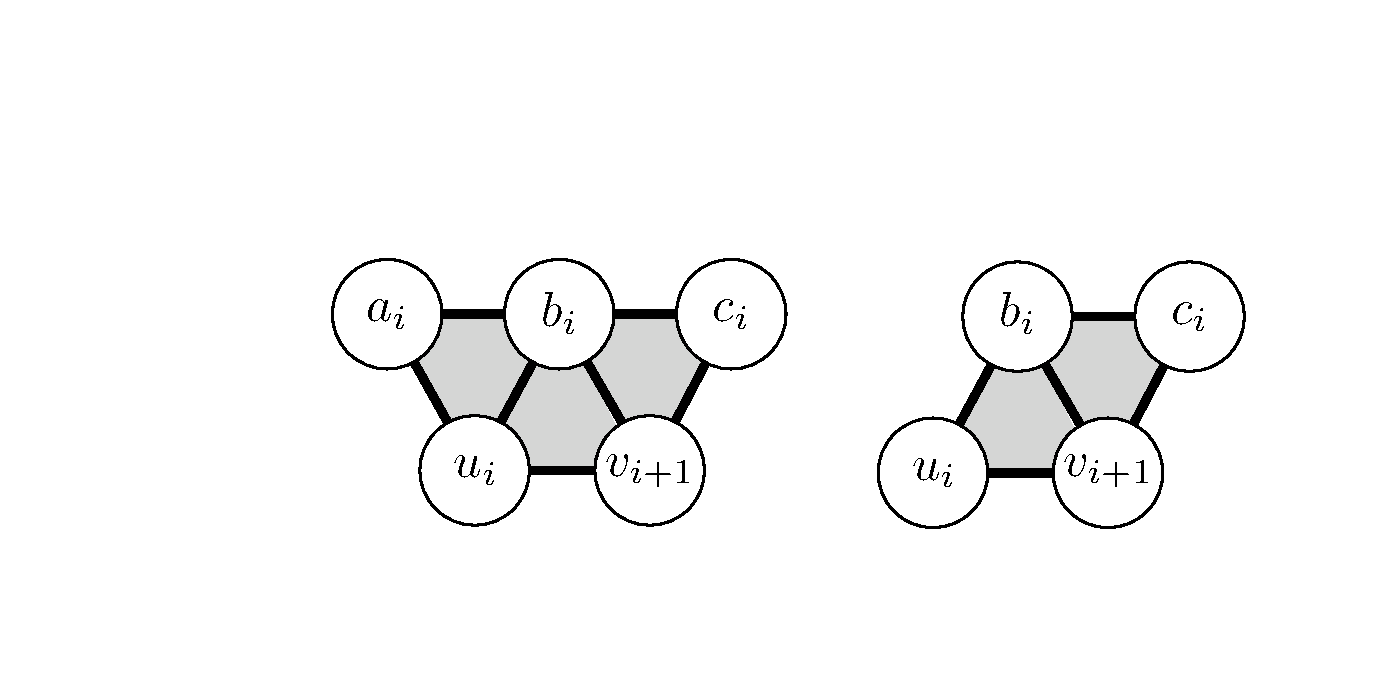
\includegraphics[width=3in]{./figures/csa-32-22.pdf}
\end{center}
\caption{The carry-save adder (CSA), or 3-2 adder, and carry-save 2-2 adder.}
\label{fig:csa-3-2}
\end{figure}

At the level of numbers, the sum of three $n$-bit numbers can be converted into
the sum of two $n$-bit numbers by applying a \emph{CSA layer} of
$n$ parallel, single-bit
CSA's. Since each CSA operates in constant depth, the entire layer also
operates in constant-depth, and we have achieved (non-modular) addition.

An important consideration here is the circuit width. The circuit above
operates out-of-place and produces two garbage qubits, the original inputs
$b_i$ and $c_i$. A single addition of three $n$-bit numbers requires a
$O(n)$ circuit width.


\section{Quantum Modular Addition}
\label{sec:csa-mod-add}

To perform addition of two numbers $a$ and $b$ modulo $m$,
we consider the variant problem of modular addition of three numbers to
two numbers:
%
%\begin{quote}
Given three $n$-bit input numbers $a$, $b$, and $c$ and an $n$-bit modulus $m$,
compute the following:
%\begin{equation}
$(u+v) = (a+b+c)[m]$,
%\end{equation}
where $(u+v)$ is a CSE number.

In this section, we provide an alternative, pedagogical explanation of
Gossett's modular reduction \cite{Gossett1998}. Later, we contribute a mapping
to a 2D architecture,
using unbounded fanout to maintain constant-depth for adding back
modular residues. This last step is missing in Gossett's original approach.

To start, we will demonstrate the basic method of modular addition and reduction
on an $n$-bit conventional number. In general, adding two $n$-bit conventional
numbers will produce an overflow $n$-bit, which we can truncate as long as
we add back its modular residue $2^n \bmod m$. How can we guarantee that we won't
generate another overflow bit by adding back the modular residue? It turns out
we can accomplish this by allowing
a slightly larger input and output number ($n+1$ bits in this case), truncating
multiple overflow bits, and adding back their modular residues.

For an $(n+1)$-bit conventional number $x$,
we truncate its high-order bits $x_n$ and $x_{n-1}$
and
add back their \emph{modular residue}, $x_{(n-1,n)}[m]$.
%
\begin{eqnarray}
x \bmod m &=& x_{(0,n)}[m] \nonumber \\
&=& x_{(0,n-2)} + x_{(n-1,n)}[m]
\end{eqnarray}
%
Since both the truncated number $x_{(0,n-2)}$ and the modular residue
are $n$-bit numbers, their sum is an $(n+1)$-bit number as desired, equivalent
to $x[m]$.

Now we must do the same modular reduction on a CSE number $(u+v)$,
which represents an $(n+1)$-bit conventional number and has
$2n$ bits.
%This is the special case mentioned in the
%previous
%section \label{star:csa-special}, where $x$ is the result of a single
%CSA layer, not repeated CSA layers alternating with truncation.
%
%Assume for now that this modular reduction works;
%in the next section we walk through an illustrated concrete example.
%We present a more formal argument in Section \ref{subsec:mod-reduce-1}.
%
First, we truncate the three high-order bits ($v_{n}, u_{n-1}, v_{n-1}$)
of $(u+v)$, yielding an $n$-bit
conventional number with a CSE representation of $2n-3$ bits:
$\{u_0, u_1, \ldots, u_{n-2}\} \cup \{v_1, v_2, \ldots, v_{n-2}\}$.
Then we add back the three modular residues
$(v_{(n)}[m], u_{(n-1)}[m], v_{(n-1)}[m])$, and we are guaranteed not to
get more overflow bits (of significance $2^{n-1}$ or higher). This equivalence
is shown in Equation \ref{eqn:mod-reduce}.
\begin{eqnarray}
(u+v)[m] &=& \left(u_{(0,n-1)} + v_{(1,n)}\right)[m] \nonumber \\
 &=& u_{(0,n-2)} +
     v_{(1,n-2)} + \nonumber \\
 & & u_{(n-1)}[m] + 
     v_{(n-1)}[m] + \nonumber \\
 & & v_{(n)}[m]
\label{eqn:mod-reduce}
\end{eqnarray}

\begin{lemma}[Modular Reduction in Constant Depth \cite{Gossett1998}]
The modular addition of three $n$-bit numbers to two $n$-bit numbers can be
accomplished
in constant depth.
\end{lemma}

\begin{proof}
Our goal is to show how to perform modular addition while keeping our numbers
of a fixed size by treating overflow bits correctly.
First, we enlarge our registers to allow the addition of $(n+2)$-bit numbers,
while keeping our modulus of size $n$ bits.
(In Gossett's original approach, he takes the equivalent step of restricting
the modulus to be of size $(n-2)$ bits.) We accomplish the modular addition
by first performing a layer of non-modular addition, truncating the three high-order
overflow bits, and then adding back modular residues controlled on these
bits in three successive layers, where we are guaranteed that no additional
overflow bits are generated.
This is illustrated for a $3$-bit modulus, and $5$-bit registers,
in Figure \ref{fig:csa-proof}.

\begin{center}
\begin{figure*}[h!tb]
\begin{displaymath}
\renewcommand\arraystretch{1.5}
\begin{array}{ccccccl}
        & a_4 & a_3 & a_2 & a_1 & a_0 & 5\text{-bit input number } a\\
        & b_4 & b_3 & b_2 & b_1 & b_0 & 5\text{-bit input number } b\\
        & c_4 & c_3 & c_2 & c_1 & c_0 & 5\text{-bit input number } c\\
\hline
        & u_4 & u_3 & u_2 & u_1 & u_0 & \text{truncate } u_{4} \\
    v_5 & v_4 & v_3 & v_2 & v_1 &     & \text{truncate } v_{4},v_{5} \\
        &     &     & c^{v_4}_2 & c^{v_4}_1 & c^{v_4}_0 & \text{add back } 2^4 \bmod m \text{ controlled on } v_4 \\
\hline
        &      & u'_3 & u'_2 & u'_1 & u'_0 & \\ 
        & v'_4 & v'_3 & v'_2 & v'_1 &      & \\
        &      &    & c^{u_4}_2 & c^{u_4}_1 & c^{u_4}_0  & \text{add back } 2^4 \bmod m \text{ controlled on } u_4 \\
\hline
        & u''_4 & u''_3 & u''_2 & u''_1 & u''_0 & \text{the bit } u''_4 \text{ is the same as } v'_4 \\
        & v''_4 & v''_3 & v''_2 & v''_1 &       &  \\
        &       &    & c^{v_5}_2 & c^{v_5}_1 & c^{v_5}_0 & \text{add back } 2^5 \bmod m \text{ controlled on } v_5 \\
\hline
        & u'''_4 & u'''_3 & u'''_2 & u'''_1 & u'''_0 & \text{ Final CSE output with } 5 \text{ bits}\\
        & v'''_4 & v'''_3 & v'''_2 & v'''_1 &        & \text{ Final CSE output with } 5 \text{ bits}\\
\end{array}
%\begin{array}{cccccccr}
%        & a_{n+1} & a_{n} & a_{n-1} & \ldots & a_1 & a_0 & \text{input number } a\\
%        & b_{n+1} & b_{n} & b_{n-1} & \ldots & b_1 & b_0 & \text{input number } b\\
%        & c_{n+1} & c_{n} & c_{n-1} & \ldots & c_1 & c_0 & \text{input number } c\\
%\hline
%        & u_{n+1} & u_{n} & u_{n-1} & \ldots & u_1 & u_0 & \text{truncate } u_{n+1} \\
%v_{n+2} & v_{n+1} & v_{n} & v_{n-1} & \ldots & v_1 & 0   & \text{truncate } v_{n+1},v_{n+2} \\
%        &         &       & x_{n-1} & \ldots & x_1 & x_0 \\
%\hline
%        &         & u'_{n} & u'_{n-1} & \ldots & u'_1 & u'_0 & \\ 
%        & v'_{n+1} & v'_{n} & v'_{n-1} & \ldots & v'_1 & 0 &  \\
%        &         &       & x_{n-1} & \ldots & x_1 & x_0 \\
%\hline
%        & u''_{n+1} & u''_{n} & u''_{n-1} & \ldots & u''_1 & u''_0 & \\
%        & v''_{n+1} & v''_{n} & v''_{n-1} & \ldots & v''_1 & 0 &  \\
%        &         &       & y_{n-1} & \ldots & y_1 & y_0 \\
%\hline
%        & u'''_{n+1} & u'''_{n} & u'''_{n-1} & \ldots & u'''_1 & u'''_0 & \\
%        & v'''_{n+1} & v'''_{n} & v'''_{n-1} & \ldots & v'''_1 & 0 &  \\
%\hline
%\end{array}
\end{displaymath}
\caption{A schematic proof of Gossett's constant-depth modular reduction for $n=3$}
\label{fig:csa-proof}
\end{figure*}
\end{center}

We use the following notation.
The non-modular sum of the first layer is $u$ and $v$.
The CSE output of the first modular reduction layer
is $u'$ and $v'$, and the modular residue is
written as $c^{v_{n+1}}$ to mean the precomputed value $2^{n+1} \bmod m$
controlled on $v_{n+1}$.
The CSE output of the second modular reduction layer
is $u''$ and $v''$, and the modular residue is written as
$c^{u_{n+1}}$ to mean the precomputed value $2^{n+1} \bmod m$
controlled on $u_{n+1}$.
The CSE output of the third and final modular reduction layer
is $u'''$ and $v'''$, and the modular residue is written as
$c^{v_{n+2}}$ to mean the precomputed value $2^{n+2} \bmod m$
controlled on $v_{n+2}$.

We show that at no layer is an overflow $(n+2)$-bit generated, namely in the
$v$ component of any CSE output. (The $u$ component will never exceed the
size of the input numbers.) First, we know that no $v'_{n+2}$ bit
is generated after the first modular reduction layer, because we have
truncated away all $(n+1)$-bits. Second, we know that no $v''_{n+2}$ bit is
generated because we only have one $(n+1)$-bit to add, $v'_{n+1}$.
Finally, we need to show a sufficient condition for no $v'''_{n+2}$ bit being
generated in the third modular reduction layer. This bit is the majority of
$u''_{n+1}$, $v''_{n+1}$, and $c^{v_{n+2}}_{n+1} = 0$. This means we only have
to guarantee that at most one of $u''_{n+1}$ and $v''_{n+1}$ has value 1.
This is equivalent to requiring that
$u''_{(n,n+1)} + v''_{(n+1)} \le 3\cdot 2^{n+1}$, that is, the sum of these
three bits has value at most $3$. Bit $u''_{n+1}$ is copied directly from
$v'_{n+1}$ by the rules of CSA, which implies the following condition for
the second modular reduction layer:
$u'_{(n)} + v'_{(n,n+1)} \le 3\cdot 2^n$. This is true because
$u'_{(n)} + v'_{(n+1)} = u_{(n)} + v_{(n)} \le 2$ and $v'_{(n)} \le 1$.
Everywhere
we use the fact that the modular residues are restricted to $n$ bits.
Therefore, the modular sum is computed as the sum of two $(n+2)$-bit numbers
with no overflows in constant-depth.
\end{proof}

As a side note, we can perform modular reduction in one layer instead of
three by decoding the three overflow bits into one of seven different
modular residues. This can also be done in constant depth, and in this case
we only need to enlarge all our registers to $(n+1)$ bits instead of $(n+2)$
as in the proof above. However, we omit this proof here for simplicity.

To summarize,
the circuit resources for modular addition are $O(1)$ depth and $O(n)$ width.

%%%%%%%%%%%%%%%%%%%%%%%%%%%%%%%%%%%%%%%%%%%%%%%%%%%%%%%%%%%%%%%%%%%%%%%%%%%%%%%
\subsection{A Concrete Example of\\ Modular Addition}
\label{subsec:concrete}

\begin{center}
\begin{figure*}[h!bt]
\centerline{
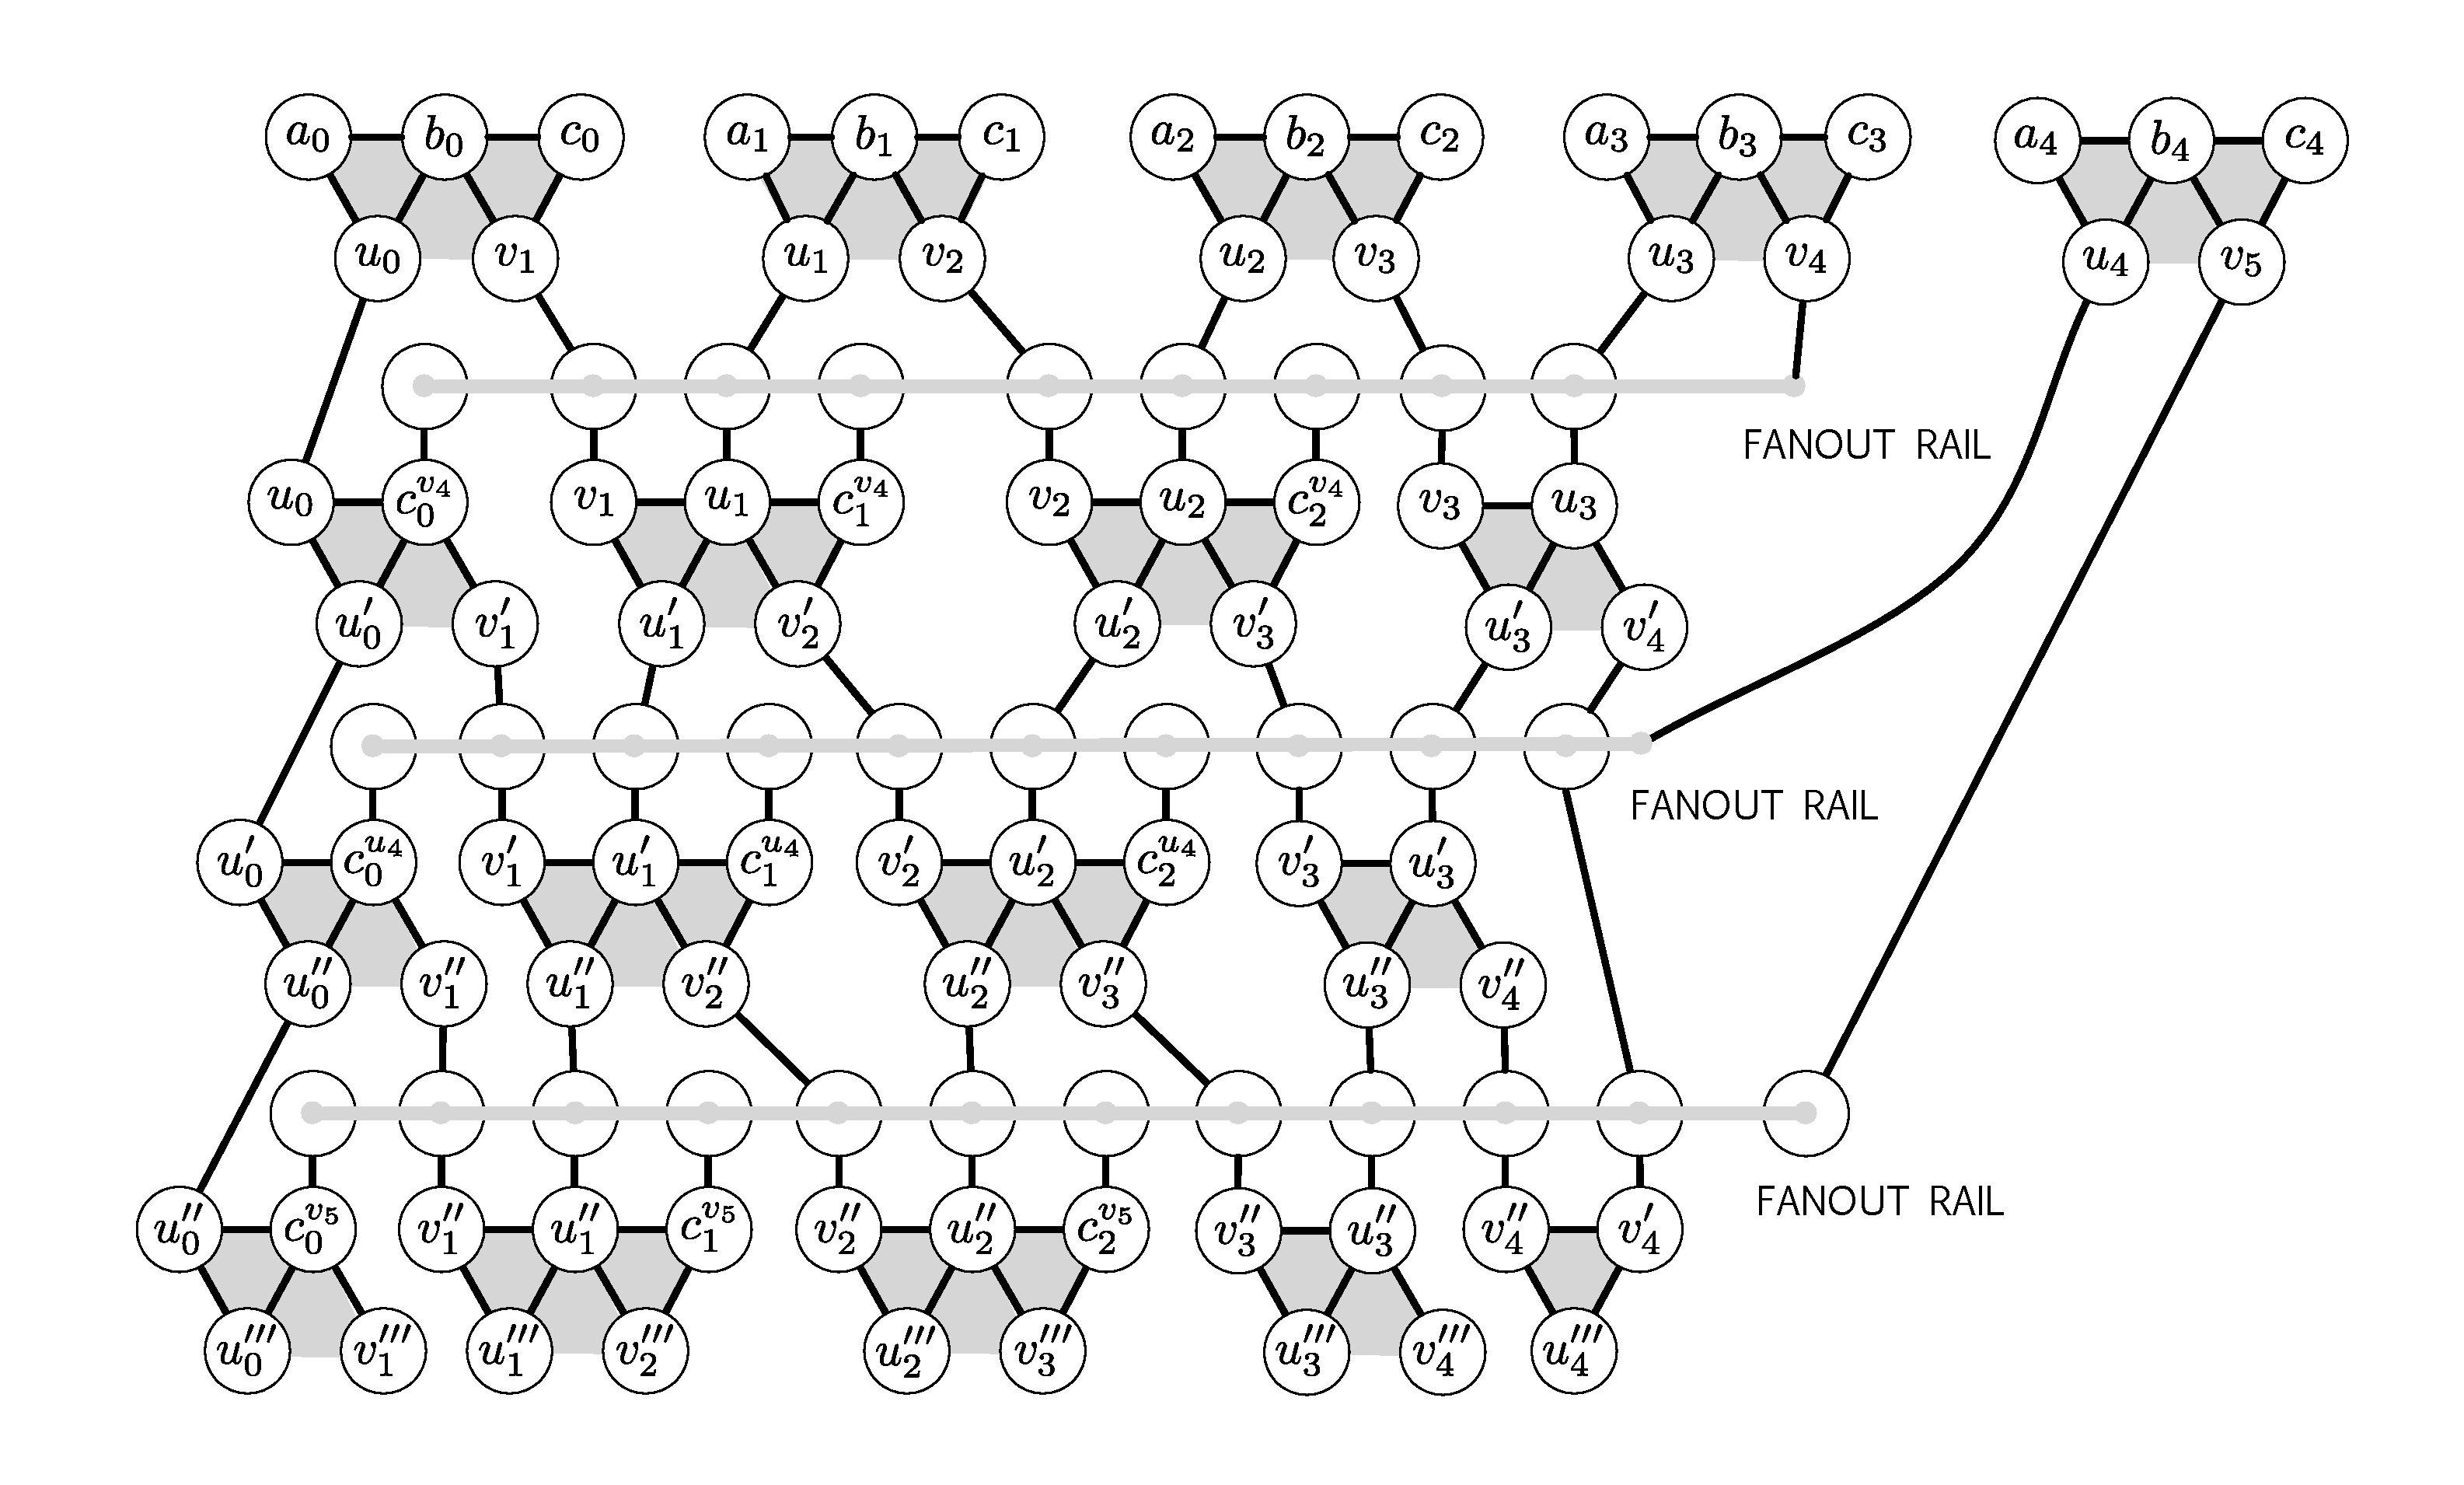
\includegraphics[width=6.5in]{./figures/mod-add-fixed.pdf}
}
\caption{Addition and three rounds of modular reduction for a 3-bit
modulus.}
\label{fig:csa-add-4}
\end{figure*}
\end{center}

A 2D circuit for modular addition of $5$-bit numbers using
four layers of parallel CSA's is shown graphically in Figure \ref{fig:csa-add-4}
which corresponds directly to the schematic proof in Figure \ref{fig:csa-proof}.
Figure \ref{fig:csa-add-4} also represents the approximate
physical layout of the qubits as they would look if this
circuit were to be fabricated.
Here, we convert the sum of three
$5$-bit integers into the modular sum of two $5$-bit integers, with a
$3$-bit modulus $m$.
In the first layer, 
we perform 4 CSA's in parallel on the input numbers ($a,b,c$) and produce the
output numbers ($u, v$).

As described above, we truncate
the three high-order bits during the initial CSA round
(bits $u_4, v_4, v_5$) to retain a $4$-bit number.
Each of these bits serves as a control for adding its modular residue to
a running total. We can classically precompute $2^4[m]$ for the two
additions controlled on $u_4$ and $v_4$ and
$2^5[m]$ for the addition controlled on $v_5$.

In layer 2,
we use a constant-depth fanout rail (see Figure \ref{fig:cd}) to
distribute the control bit $v_4$ to its modular residue, which we denote as
%%\begin{equation}
$\ket{c^{v_4}} \equiv \ket{2^4[m]\cdot v_4}$.
%%\end{equation}
%This fanout requires constant depth;
$c^{v_4}$ has $n$ bits, which we add to the CSE results of layer 1.
The results $u_i$ and $v_{i+1}$ are teleported into layer 3. The exception is
$v'_4$ which is teleported into layer 4, since there are no other $4$-bits
to which it can be added. Wherever there are only
two bits of the same significance, we use the 2-2 adder from \ref{sec:csa}.

Layer 3
%%, shown in Figure \ref{fig:csa-add-3},
operates similarly to layer 2, except that the modular residue is controlled on
$u_4$:
%%\begin{equation}
$\ket{c^{u_4}} \equiv \ket{2^4[m] \cdot u_4}$.
%%\end{equation}
%This fanout again requires constant depth; 
$c^{u_4}$ has $3$ bits, which we
add to the CSE results of layer 2, where $u'_i$ and $v'_{i+1}$ are teleported
forward into layer 4.

Layer 4
%%, shown in Figure \ref{fig:csa-add-4},
is similar to layers 2 and 3, with the modular residue controlled on $v_5$:
%%\begin{equation}
$\ket{c^{v_5}} \equiv \ket{2^5[m] \cdot v_5}$.
%%\end{equation}
%This fanout is constant depth; 
$c^{v_5}$ has $3$ bits, which we
add to the CSE results of layer 3.
There is no overflow bit $v'''_5$, and no carry bit from $v''_4$ and $v'_4$
as argued in Lemma 1.
The final modular sum $(a+b+c)[m]$ is $u'''+v'''$.


\section{Quantum Modular\\ Multiplication}
\label{sec:csa-mod-mult}

We can build upon our carry-save adder to implement quantum modular
multiplication in logarithmic depth. We start with a completely classical
problem to illustrate the principle of multiplication by repeated addition.
Then we consider modular multiplication of two quantum numbers in a serial
and a parallel fashion in
\ref{subsec:csa-mod-mult-qq}. Both of these problems use as a subroutine the
generic problem of \emph{modular multiple addition} which we define and solve
in \ref{subsec:mma}.

%%%%%%%%%%%%%%%%%%%%%%%%%%%%%%%%%%%%%%%%%%%%%%%%%%%%%%%%%%%%%%%%%%%%%%%%%%%%%%%
First we consider a completely classical problem:
given three $n$-bit classical numbers $a$, $b$, and $m$,
compute $c = ab \bmod m$, where $c$ is allowed to be in CSE.

We only have to add shifted
multiples of $a$ to itself, ``controlled'' on the bits of $b$. There are
$n$ shifted multiples of $a$, let's call them $z^{(i)}$, one for every bit of $b$:
%%\begin{equation}
$z^{(i)} = 2^i a b_i \bmod m$.
%%\end{equation}
We can parallelize the addition of $n$ numbers in a logarithmic depth
binary tree to get a total depth of $O(\log n)$.

%%%%%%%%%%%%%%%%%%%%%%%%%%%%%%%%%%%%%%%%%%%%%%%%%%%%%%%%%%%%%%%%%%%%%%%%%%%%%%
\subsection{Modular Multiplication of\\ Two Quantum Numbers}
\label{subsec:csa-mod-mult-qq}

We now consider the problem of multiplying a classical number controlled
on a quantum bit and a
\emph{quantum number},\footnote{In this paper, quantum
numbers often result by entangling a classical number in one register with a
quantum control bit. This should not be confused with the physics meaning
of a quantum number.} which is a
quantum superposition of classical numbers:
%\begin{quote}
given an $n$-qubit quantum number $\ket{x}$, a control qubit $\ket{p}$,
and two $n$-bit classical numbers $a$
and $m$,
compute $\ket{c} = \ket{xa[m]}$, where $c$ is allowed to be in CSE.
This problem occurs naturally in modular exponentiation (described in
the next section) and can be considered \emph{serial multiplication},
in that $t$ quantum numbers are multiplied in series to a single
quantum register.
%\end{quote}

We first create $n$ quantum numbers $\ket{z^{(i)}}$,
which are shifted multiples of the classical number $a$ controlled on the bits
of $x$:
%\begin{equation}
$\ket{z^{(i)}} \equiv \ket{2^i a[m] \cdot x_i }$.
%\end{equation}
How do we create these numbers, and what is the depth of the procedure?
First, note that $\ket{2^i a[m]}$ is a classical number, so we can
precompute this classically and prepare them in parallel using single-qubit
operations
on $n$ registers, each consisting of $n$ ancillae qubits. Each $n$-qubit
register will hold a future $\ket{z^{(i)}}$ value.
We then copy all
$n$ bits of $x$, $n$ times each, using an unbounded fanout operation so that
$n$ copies of each bit $\ket{x_i}$ is next to register $\ket{z^{(i)}}$.
This takes a total of $O(n^2)$ parallel CNOT operations.
We then entangle each $\ket{z^{(i)}}$ with the corresponding $x_i$.
The schematic for this is shown in Figure \ref{fig:mod-mult-create}, not
showing how we interleave these numbers into groups of three using
constant-depth teleportation. This reduces to the task of modular
multiple addition, in order to add these numbers down to a single
number modulo $m$, which is described in \ref{subsec:mma}.

\begin{figure*}[htp!]
\centerline{
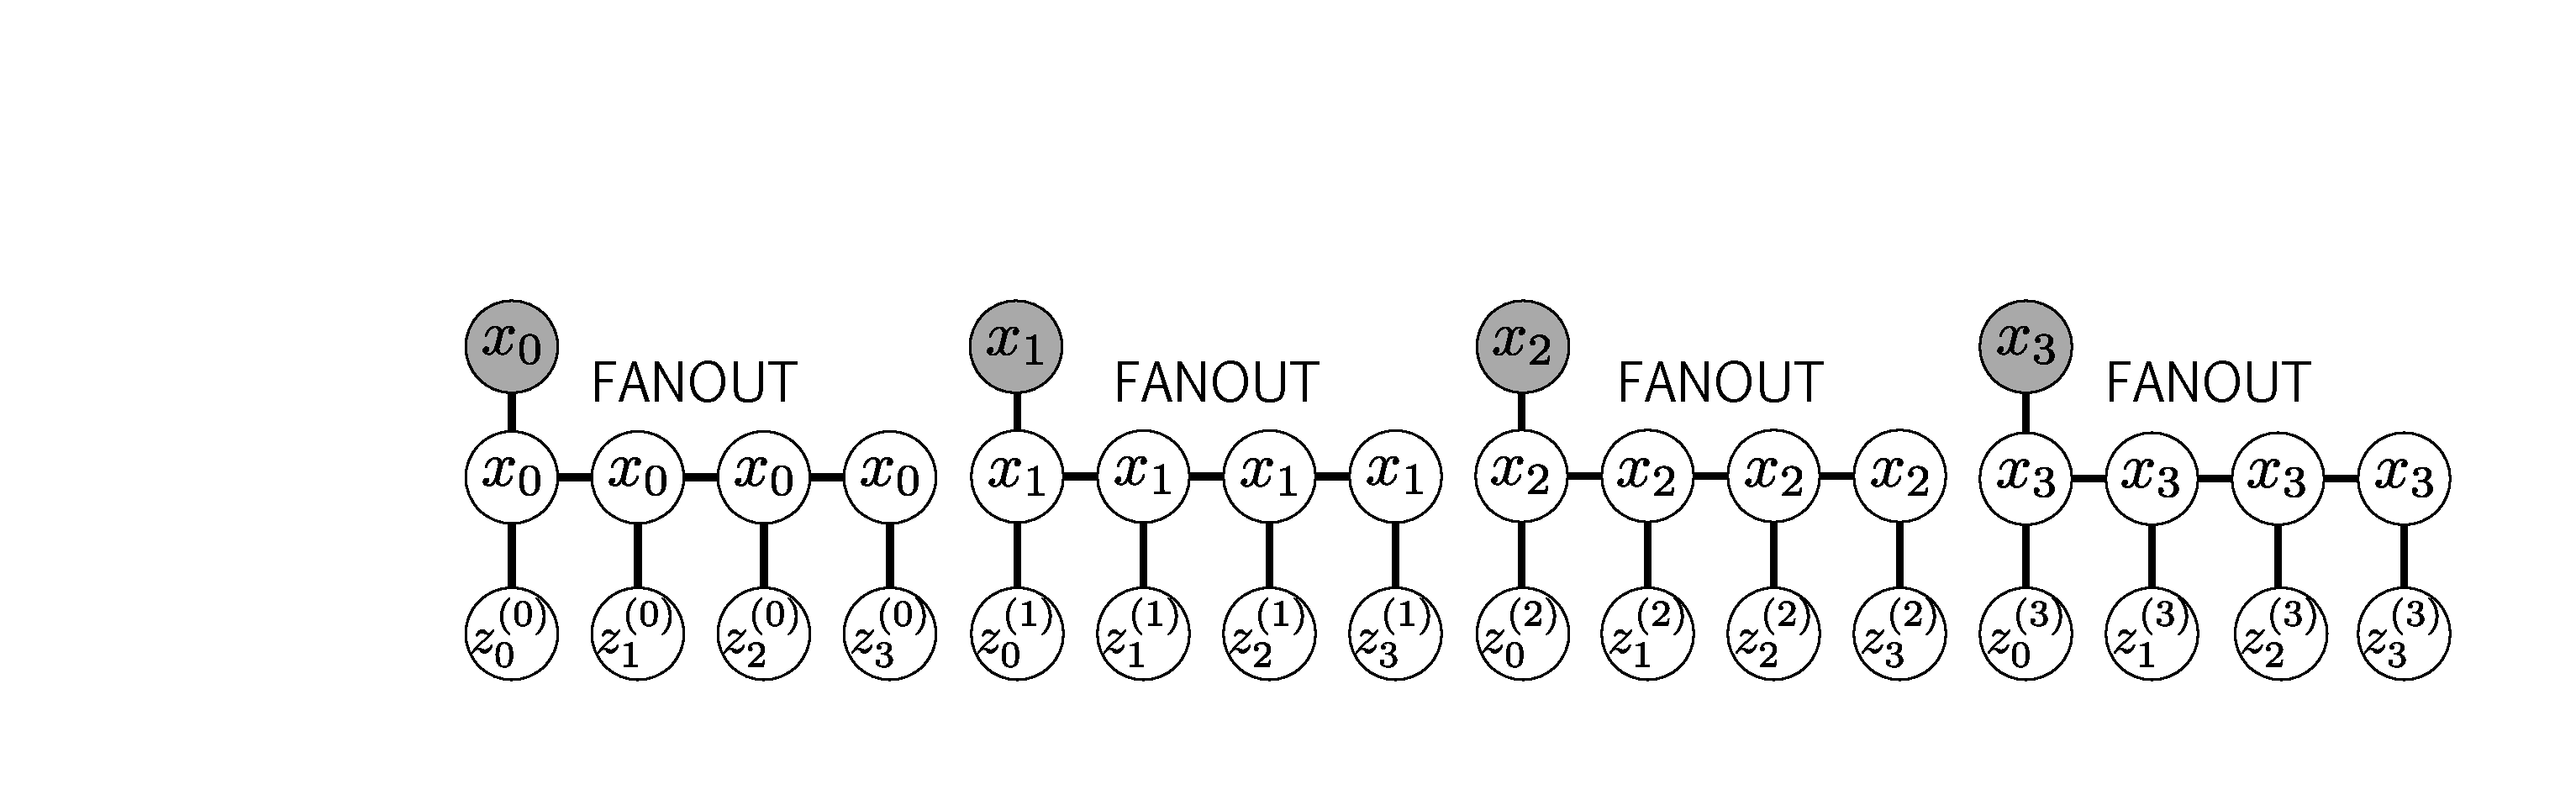
\includegraphics[width=4.5in]{figures/znumbers.pdf}
}
\caption{Creating $n=4$ shifted values $\{z^{(0)},z^{(1)},z^{(2)},z^{(3)}\}$
for an input number $x$.}
\label{fig:mod-mult-create}
\end{figure*}

Finally, we tackle the most interesting problem:
%\begin{quote}
given two $n$-qubit quantum numbers $\ket{x}$ and
$\ket{y}$ and a $n$-bit classical number
$m$,
compute $\ket{c} = \ket{xy \bmod m}$,
where $\ket{c}$ is allowed to be in CSE.
This can be considered \emph{parallel multiplication} and is responsible
for our logarithmic speedup in modular exponentiation.
%\end{quote}

Instead of creating $n$ quantum numbers $\ket{z^{(i)}}$, we must create
$n^2$ numbers
$\ket{z^{i,j}}$ for all possible pairs of quantum bits $x_i$ and $y_j$,
$i,j \in \{0,\ldots,n-1\}$:
%\begin{equation}
$\ket{z^{i,j}} \equiv \ket{2^i2^j[m]\cdot x_i \cdot y_j}$.
%\end{equation}
We create these numbers using a similar procedure to the previous problem.
Adding $n^2$ quantum numbers of $n$ qubits each takes depth
$O(\log(n^2))$ which is still $O(\log n)$.
Creating $n^2\times n$-bit quantum numbers takes width $O(n^3)$. 

%%%%%%%%%%%%%%%%%%%%%%%%%%%%%%%%%%%%%%%%%%%%%%%%%%%%%%%%%%%%%%%%%%%%%%%%%%%%%%%
\subsection{Modular Multiple Addition}
\label{subsec:mma}

As a subroutine to modular multiplication, we define the operation of
repeatedly adding multiple numbers down to a single CSE number, called
\emph{modular multiple addition}.

The modular multiple addition circuit generically adds down $t\times n$-bit
conventional numbers to an $n$-bit CSE number.
%
\begin{equation}
z^{(0)} + z^{(1)} + \ldots z^{(n-1)} \equiv (u+v)[m]
\end{equation}
%
It does not matter how the
$t$ numbers are generated, as long as they are divided into groups of three
and have their bits interleaved to be the inputs of a CSA tile.
In the cases above, serial multiplication results in
$t = n$ and parallel multiplication results in $t = n^2$.
At the beginning of the circuit, all CSA tiles are
\emph{active} in that they have tile input numbers $z^{(i)}$
to multiply, and their tile outputs will affect the overall circuit output,
$u+v$.

As the circuit proceeds through a number of timesteps,
tiles will become \emph{inactive} when they
do not receive new numbers for their tile inputs; at
that point, their tile outputs can no longer affect the circuit output.
Since the CSA tile is a 3-2 adder, one can see that if there are $t$ CSA tiles
active at the beginning of a timestep, there are $\lceil 2t/3 \rceil$ active
tiles at the end of the timestep, since there are roughly two-thirds as many
input numbers left to add down to the circuit output $u+v$. One can see that
the total number of timesteps
is therefore $\lceil \log_{3/2}(t/3) \rceil + 1$.

To facilitate the below discussion, we will assign colors to each CSA tile,
which are updated during the circuit execution. Active tiles can either be
black or gray.
A \emph{black} tile will keep its two output numbers as inputs and receive
a third input number. An exception is the rightmost black tile may teleport
one of its output numbers to its left black nearest neighbor and receive
two input numbers from its right gray nearest neighbor.
A \emph{gray} tile will teleport one of its output
numbers to the nearest active tile to its left and the other output number
to the nearest active tile to its right. An exception is the rightmost gray
tile may teleport both output numbers to its left black nearest neighbor.
We can think of inactive tiles as
\emph{white} tiles in that they ``fade'' out of the circuit, and numbers
get teleported through them without stopping to be added. The symbols for
these colors are shown in Figure \ref{fig:tile-colors}.

\begin{figure*}[htb!]
\centerline{
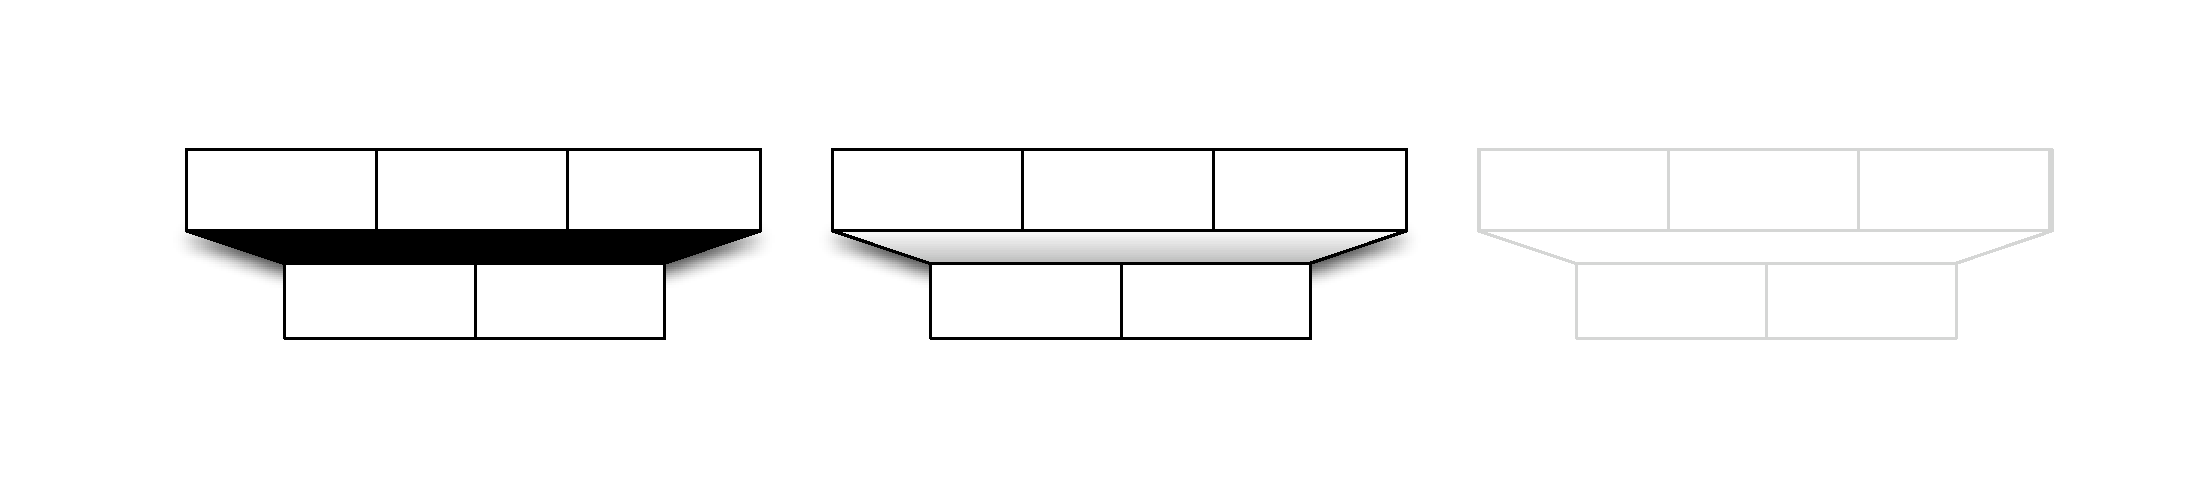
\includegraphics[width=5.5in]{figures/csa-tile-colors.pdf}
}
\caption{From left to right, the symbols for a black, gray, and white tile,
respectively.}
\label{fig:tile-colors}
\end{figure*}


The rules for
updating tiles at the end of each timestep are as follows:

\begin{itemize}
\item \textbf{Black tiles} are always active for the next timestep, but
change colors as follows.
\begin{itemize}
\item The leftmost tile always stays black.
\item If a black tile has a gray tile as its nearest active right neighbor in
the current timestep,
it stays \textbf{black} in the next timestep.
\item If a black tile has a black tile as its nearest active neighbor either
to the right or the left, and it is not the leftmost tile,
it turns \textbf{gray} in the next timestep.
\end{itemize}
\item \textbf{Gray tiles} always turn white (inactive) in the next timestep.
\end{itemize}

The initial state of the tile colors depends on its index
$i \in \{0, 1, \ldots, q-1\}$ within $q = \lceil t/3 \rceil$ tiles.

\begin{itemize}
\item If $i \bmod 3 = 0$, then it starts out black.
\item If $i \bmod 3 = 1$, then it starts out gray.
\item If $i \bmod 3 = 2$, then it starts out black.
\end{itemize}

Given the rules above, one can see that the leftmost tile stays black
throughout the entire circuit, and holds the final output number $(u+v)$ at
the end.

Each timestep of the circuit consists of the following operations:

\begin{enumerate}
\item
All active CSA tiles will execute in
parallel to transform their three input numbers into two output numbers
(a CSE number).
\item
Gray tiles teleport their output numbers to the left and to the right to
their black tile neighbors. The exception is the rightmost gray tile will
teleport both of its output numbers to its left black tile nearest neighbor.
\item
Tile colors will change according to the rules above. Approximately
two-thirds of the tiles will
become inactive in the next timestep.
\item
Go back to Step 1 for the next timestep.
\end{enumerate}

These steps and the above tile color rules are best illustrated with a concrete
example. In Figure \ref{fig:mod-mult}, we see the circuit for modular
multiple addition as a series of
snapshots, separated by heavy dotted lines, with the passage of time going
downward. The tiles change color over time, and the arrows indicate the
teleportation of output numbers to neighboring active tiles in each timestep.
In the initial timestep, the tiles are numbered to show how they are assigned
their initial color.
Between Timestep 0 and Timestep 1,
all $\lceil n/3 \rceil$ CSA tiles are active. After each succeeding timestep,
$\lfloor 2/3 \rfloor$
fewer CSA tiles are active until the very end, when only one CSA tile is
active. By the convention established above,
we teleport the rightmost output numbers to the left, so that the
final output is read out from the leftmost CSA tile.

\begin{figure*}[htb!]
\centerline{
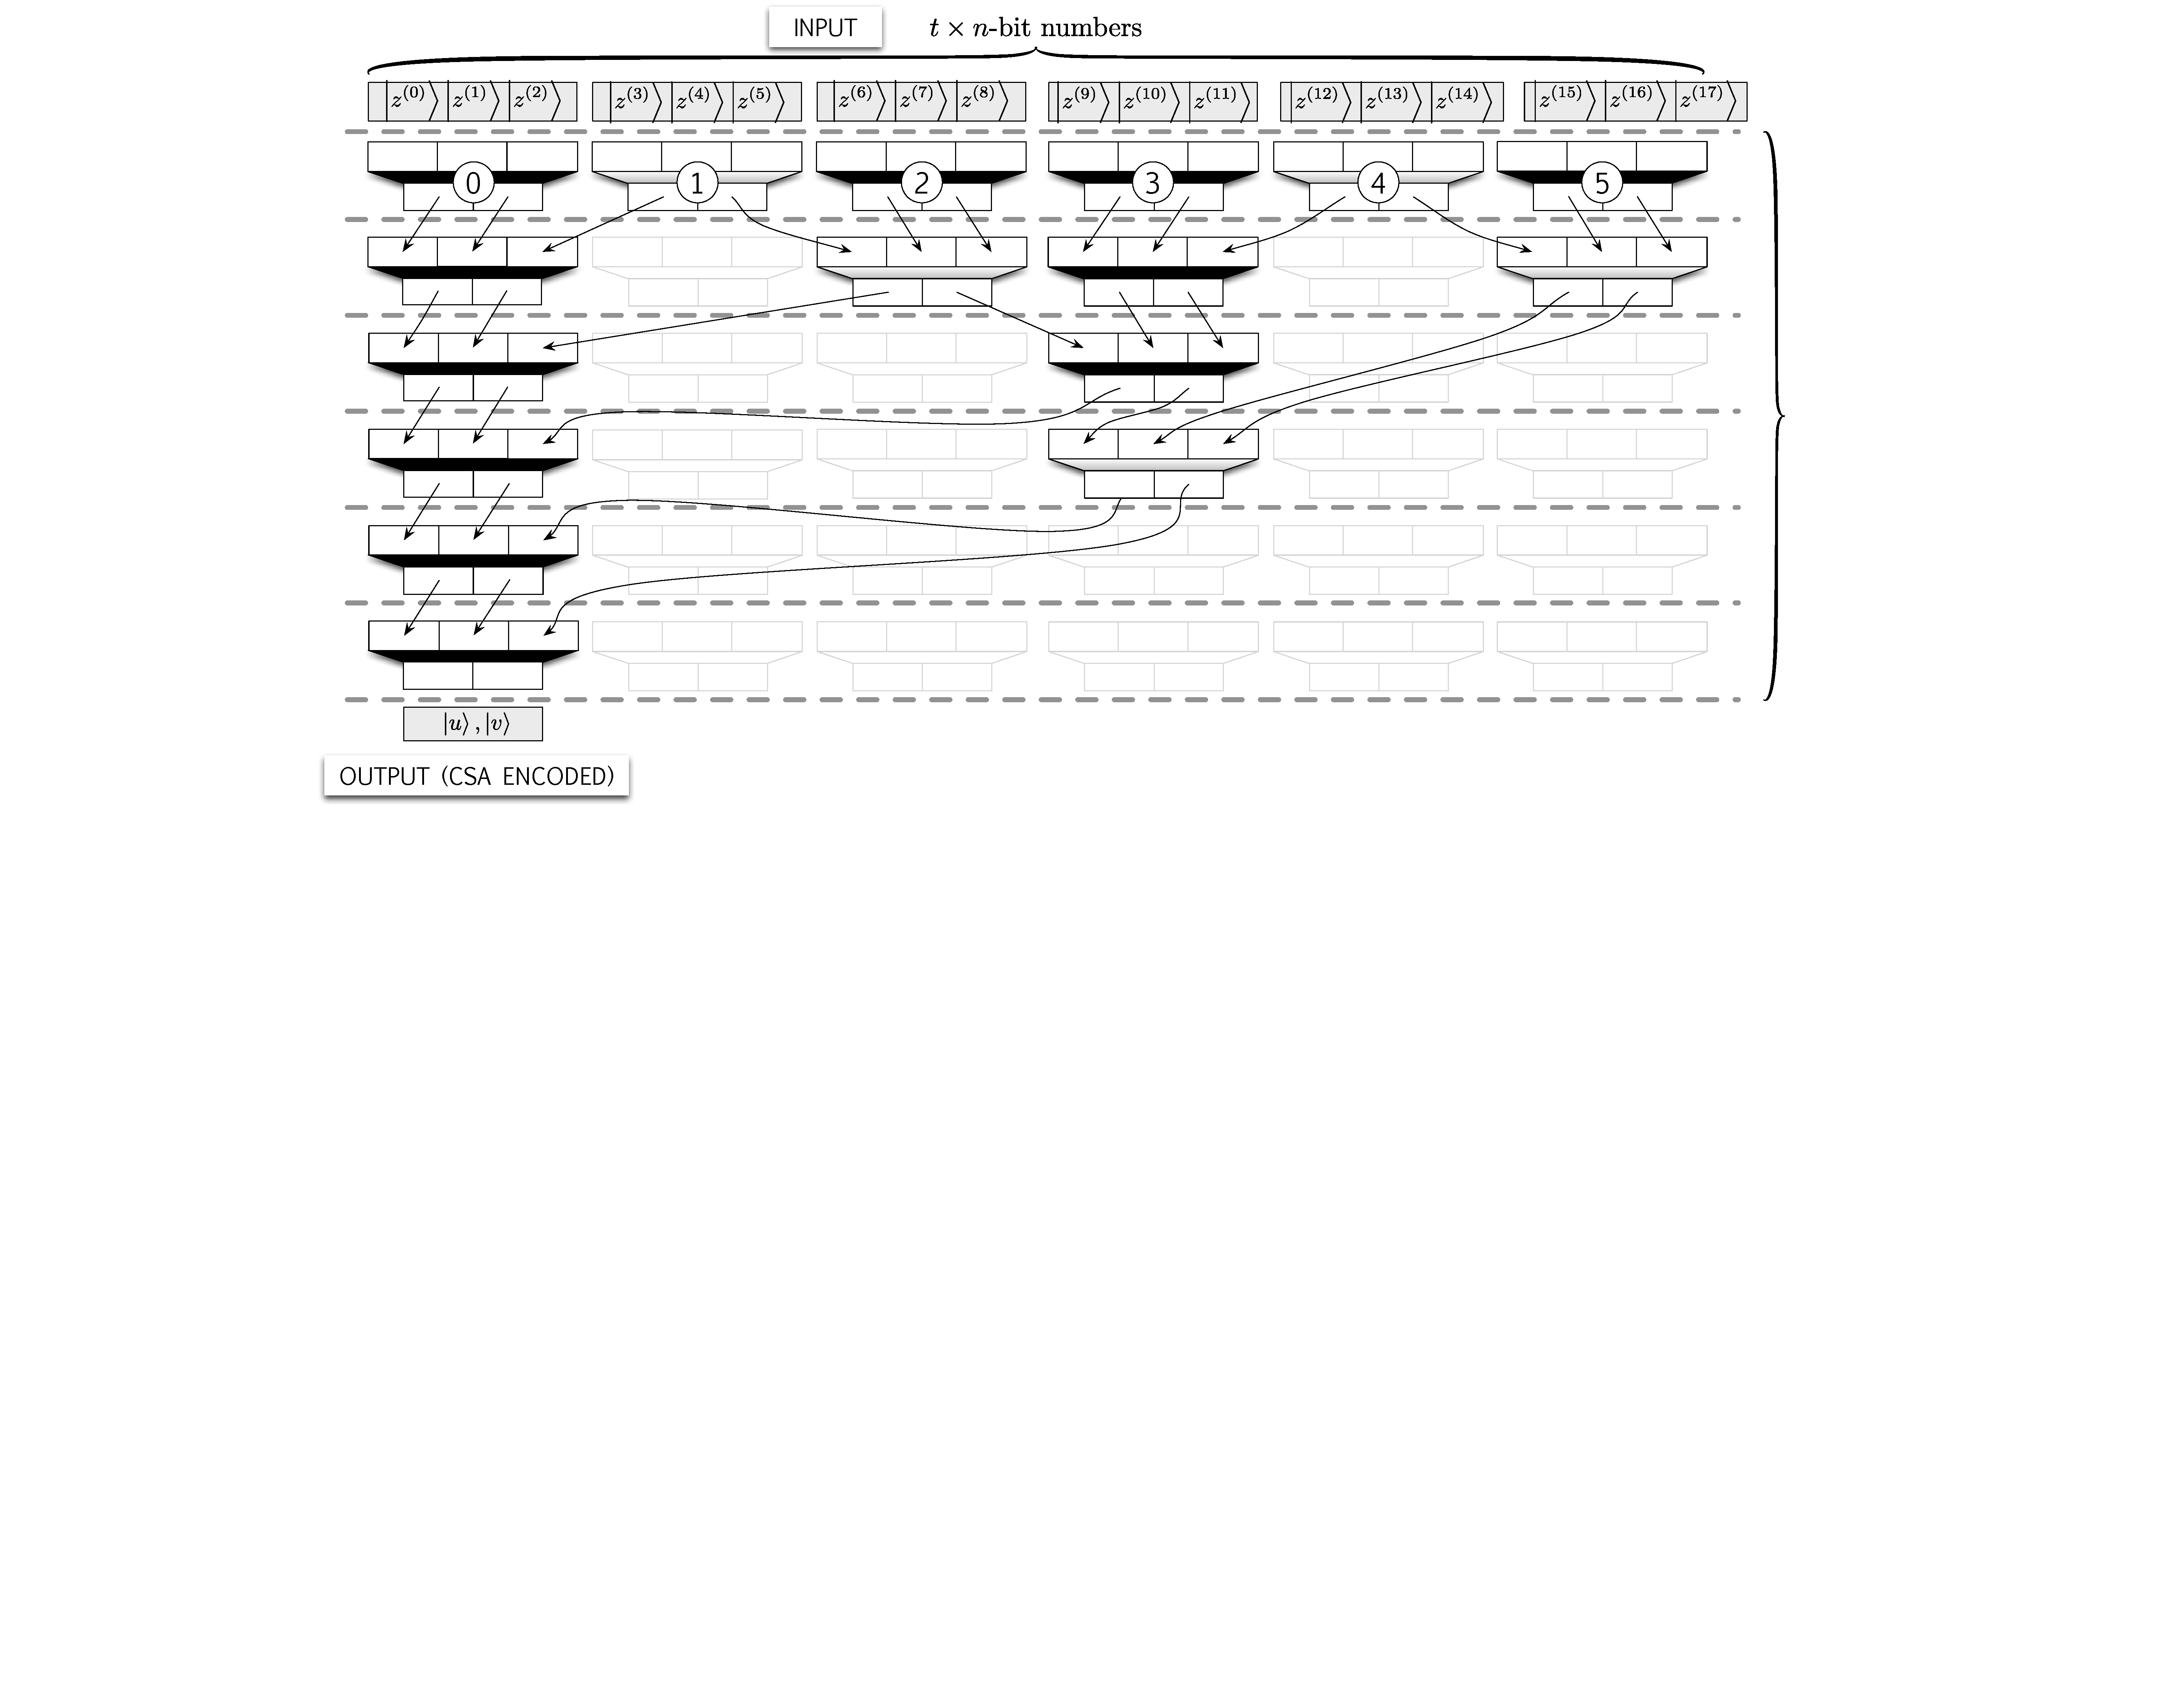
\includegraphics[width=5.5in]{figures/mod-mult-add.pdf}
}
\caption{Modular multiple addition of quantum numbers on a CSA tile
architecture for $t=18$ with depth $(\lceil \log_{\frac{3}{2}}(t/3) \rceil + 1) = 6$
timesteps}
\label{fig:mod-mult}
\end{figure*}
%

Now we can analyze the circuit resources for multiplying $n$-bit
quantum numbers, which requires $(t-2)$ modular additions, for $t=n^2$.
The circuit width is the sum of the $O(n^3)$ ancillae
needed for number generation and the ancillae required for $O(n^2)$
modular additions. Each modular addition has width $O(n)$ and depth $O(1)$
from the previous
section. There are
$\lceil \log_{3/2}(n^2 / 3) \rceil +1 $ timesteps of modular addition. Therefore
the entire modular multiplier circuit has depth $O(\log n)$ and width $O(n^3)$.


\section{Quantum Modular\\ Exponentiation}
\label{sec:modexp}

We now extend our arithmetic to modular exponentiation, which is repeated
modular multiplication controlled on qubits supplied by a phase estimation
procedure.
If we wish to multiply a $n$-qubit quantum input number $\ket{x}$ by
$t$ classical numbers $a^{(j)}$, we can multiply them in series.
% as shown in
%Figure \ref{fig:modexp-qc-series}.
This requires depth $O(t\log n)$ based on the modular multipliers in previous
sections.

%\begin{figure}[htp!]
%\begin{center}
%\includegraphics[width=5.5in]{figures/modexp-qc-series.pdf}
%\end{center}
%\caption{Multiplying a quantum number $\ket{x}$ by $t$ classical numbers
%$\{a^{0}, a^{1}, \ldots, a^{n-1}\}$ in series.}
%\label{fig:modexp-qc-series}
%\end{figure}

Now consider the same procedure, but this time each classical number $a^{(j)}$
is controlled on a quantum bit $p_j$. This is a special case of
multiplying by $t$ quantum numbers in series, since a classical number
entangled with a quantum number is also quantum.
%This is shown in
%Figure \ref{fig:modexp-qq-series}.
It takes the same depth $O(t\log n)$ as the previous case.
%
%\begin{figure}[htp!]
%\begin{center}
%\includegraphics[width=5.5in]{figures/modexp-qq-series.pdf}
%\end{center}
%\caption{Multiplying a quantum number $\ket{x}$ by $t$ quantum numbers
%$\{\ket{a^{0}p_0}, \ket{a^{1}p_1}, \ldots, \ket{a^{n-1}p_{n-1}}\}$ in series.}
%\label{fig:modexp-qq-series}
%\end{figure}

Finally, we consider multiplying $t$ quantum numbers
$\{x^{(0)}, x^{(1)}, \ldots, x^{(n-1)}\}$ in a parallel,
logarithmic depth, binary tree.
This is shown in Figure \ref{fig:modexp-qq-parallel}.
The tree has depth $\log_2(t)$ in modular multiplier operations. Furthermore,
each
modular multiplier operation has depth $O(\log(n))$ for $n$-qubit
numbers. Therefore, the overall depth of this parallel modular exponentiation
structure is $O(\log(t)\log(n))$. In phase estimation for QPF, it is
sufficient to take $t = O(n)$ \cite{Nielsen2000,Kitaev2002}. Therefore our total depth is
$O(\log^2(n))$ as desired. At this point, combined with the parallel phase
estimation procedure of \cite{Kitaev2002}, we have a complete factoring
implementation in our 2D nearest-neighbor architecture.
%
\begin{figure*}[tb!]
\centerline{
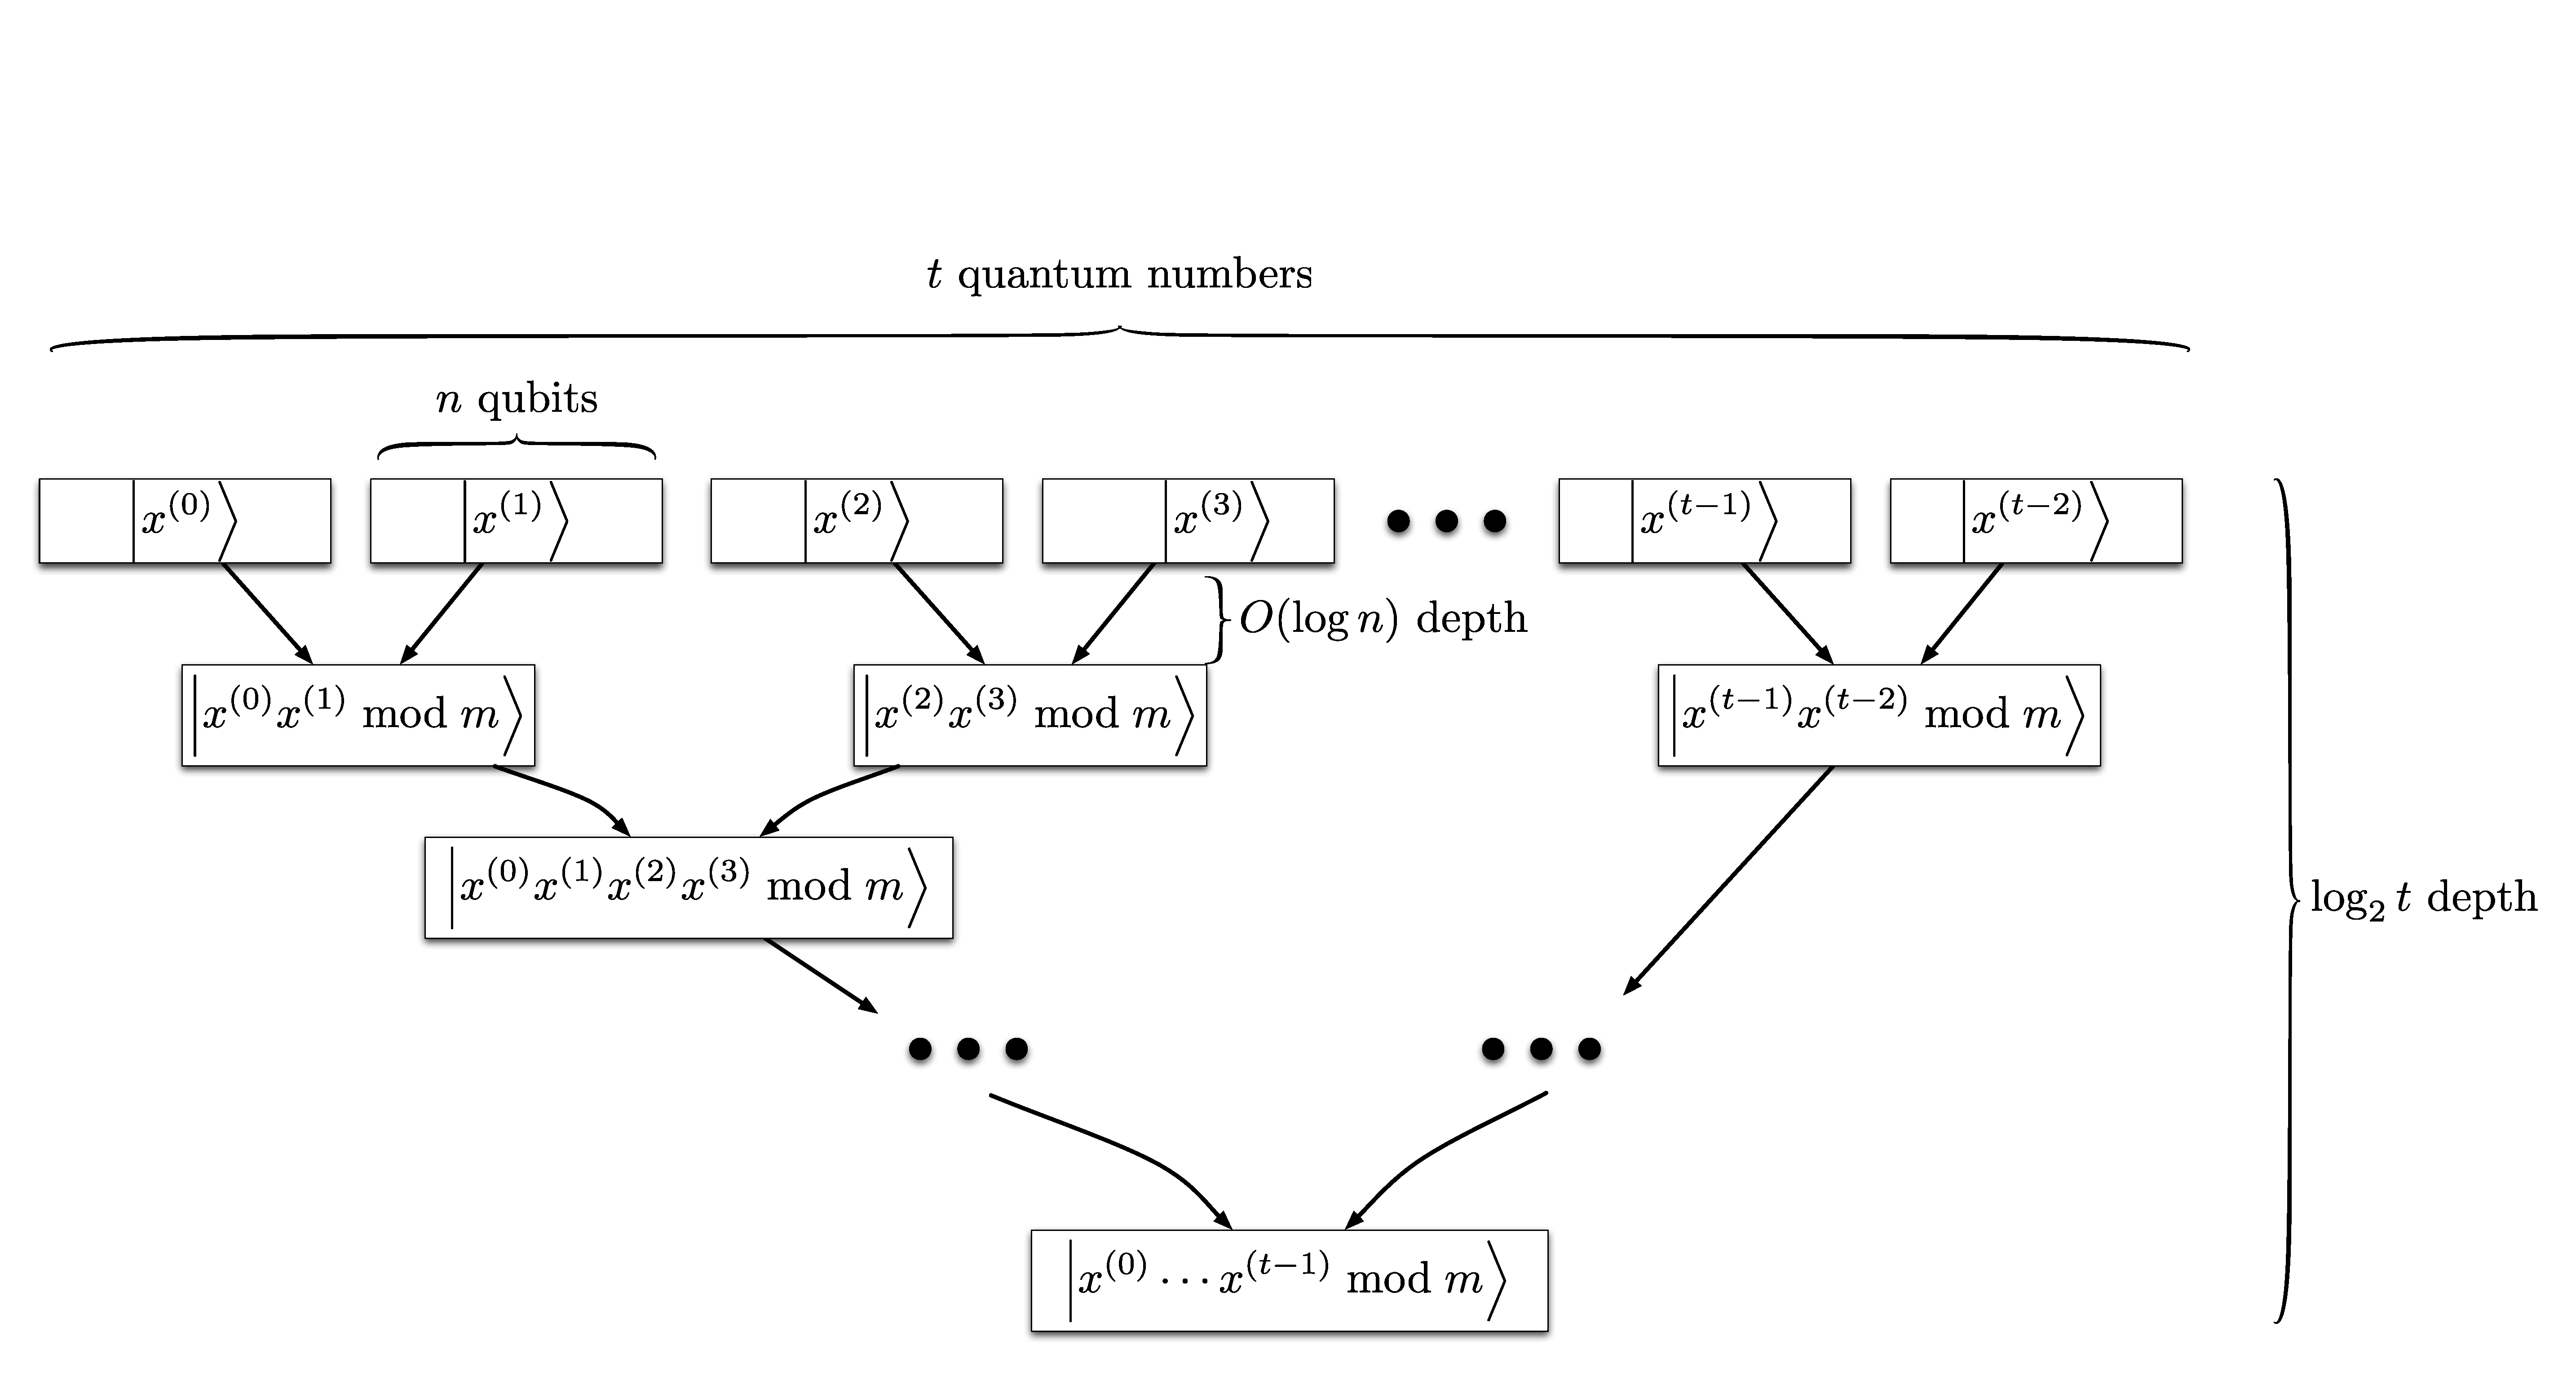
\includegraphics[width=5.5in]{figures/mod-exp-par.pdf}
}
\caption{Parallel modular exponentiation: multiplying $t$ quantum numbers
%$\{\ket{x^{(0)}}, \ket{x^{(1)}}, \ldots, \ket{x^{(t-1)}}\}$ in parallel,
in a $O(\log{(t)}\log{(n)})$-depth binary tree.}
\label{fig:modexp-qq-parallel}
\end{figure*} 

For all known QPF procedures, there are $t=O(n)$ control bits needed, and
also $O(n)$ modular multiplications in a tree of depth $O(\log n)$.
Each modular multiplication has
depth $O(\log n)$ and width $O(n^3)$.
Therefore, the depth of the parallel modular exponentiation circuit above
is $O(\log^2 n)$ and the width is $O(n^4)$.


\section{Results}
\label{sec:results}

The resources required for our approach,
as well as other nearest-neighbor approaches,
are listed in Table \ref{tab:results},
where the asymptotic resource bounds assume some fixed constant error
probability for each round of period-finding.
%, say $\epsilon=1/4$.
% and $\delta' = 1/2$ for KSV-QPF.
%Note that the
%number of measurements are included for completeness.
%, since these are
%not counted as gates in our model but may be comparable in terms of
%execution time.
%Some table cells are blank if the entries are not relevant to the current comparison, or if the entires were not %calculated in the prior work.
We achieve an exponential
improvement in nearest-neighbor circuit depth (from quadratic to polylogarithmic)
with our approach at the cost of a polynomial increase in
circuit width. Similar depth improvements at the cost of width increases can be achieved using the modular multipliers
of other factoring implementations
by arranging them in a parallel, KSV-style modular exponentiator.
%
\begin{table*}[htb!]
\begin{center}
\begin{tabular}{|c|c|c|c|}
\hline
Implementation             & Architecture      & Depth             & Width     \\
\hline
Vedral, Barenco \& Ekert \cite{Vedral1996}   & \textsc{AC}       & $O(n^3)$      & $O(n)$ \\
Gossett \cite{Gossett1998}                   & \textsc{AC}       & $O(n \log n)$ & $O(n^2)$  \\
Beauregard \cite{Beauregard2002}                & \textsc{AC}       & $O(n^3)$      & $O(n)$ \\
Zalka \cite{Zalka1998}                     & \textsc{AC}       & $O(n^2)$      & $O(n)$     \\
Takahashi \& Kunihiro \cite{Takahashi2006}     & \textsc{AC}       & $O(n^3)$      & $O(n)$ \\
%Cleve \& Watrous           & \textsc{AC}       & $O(\log L)$   & $O(L)$ \\
\hline
Fowler, Devitt, Hollenberg \cite{Fowler2004} & \textsc{1D NTC}   & $O(n^4)$ & $O(n^3)$\\
% + 40L^3 + 58L^2 + 2L - 2$ & $32L^3 + 80 L^2 - 4L - 2$ \\
Kutin \cite{Kutin2006}                     & \textsc{1D NTC}   & $O(n^2)$ & $O(n)$\\
\hline
%$18L^2 + 12L\log_2^2 L + O(L \log L) $ & $3L + 2\log_2 L + 2$ \\
Current Work               & \textsc{2D NTC}   & $O(\log^2{n})$ & $O(n^4)$   \\
\hline
\end{tabular}
\end{center}
\caption{Asymptotic resource usage for quantum factoring of an $n$-bit number.}
\label{tab:results}
\end{table*}


\section{Conclusions and Future Work}
\label{sec:conclude}

In this paper, we have presented a 2D architecture for factoring on a quantum
computer.
%While this is only an intermediate progress report, the preliminary
%results are promising.
Using a combination of algorithmic
improvements (carry-save adders and parallelized phase estimation) 
and architectural improvements (irregular two-dimensional layouts and
constant-depth communication), we conclude
that we can run
the central part of Shor's factoring algorithm (quantum period-finding)
with asymptotically smaller depth than previous implementations.
%, both
%asymptotically and numerically.

%We also provide a constructive upper bound on the overhead
%of nearest-neighbor (NTC) architectures over AC architectures.
%The best-known depth for factoring has constant-depth, but it is an open
%question whether we can satisfy the nearest-neighbor constraint while
%maintaining this constant depth. Furthermore, the cost of decreasing depth
%is often that of increasing width or size, and this time-space tradeoff is
%currently not very well known both for the current work and other
%implementations mentioned in Section \ref{sec:related}.
%Characterizing these tradeoffs is the most obvious extension to
%the current work.

For future work, we would like to determine the exact width, depth, and size of
our proposed factoring circuit, including the constants, as well as
further optimizing our depth to be constant.
%We would also like to determine how our approach compares to the constant-depth
%results in \cite{Browne2009} in terms of circuit size and width.
Along those lines, Rosenbaum recently showed how to convert any $n$-qubit CCAC
circuit to an equivalent CCNTC circuit in constant depth using $n^2$ ancillae
\cite{Rosenbaum2012}.
It is an interesting open question how a
generic conversion of a constant-depth CCAC factoring architecture
\cite{Browne2009,Hoyer2002} to CCNTC compares to our hand-optimized circuit.
The depth of our circuit may also be improved by extending the carry-save adder
from
a $3\rightarrow 2$ circuit to any $2^{n-1}\rightarrow n$ circuit.

The authors wish to thank Aram Harrow, Austin Fowler, and David Rosenbaum for
useful discussions.
P. Pham conducted the factoring part of this work during
an internship at Microsoft Research.
He also acknowledges funding of the architecture and layout portions
of this work from
the Intelligence Advanced Research Projects Activity
(IARPA) via Department of Interior National Business Center contract
number D11PC20167. The U.S. Government is authorized to reproduce and
distribute reprints for Governmental purposes notwithstanding any
copyright annotation thereon. Disclaimer: The views and conclusions
contained herein are those of the authors and should not be
interpreted as necessarily representing the official policies or
endorsements, either expressed or implied, of IARPA, DoI/NBC, or the
U.S. Government.


\bibliography{factor2d}
\bibliographystyle{tocplain}

\end{document}
